\documentclass[12pt]{article}
\usepackage{a4}
\usepackage[german]{babel}
\setlength{\parindent}{0.35cm}
\pagestyle{headings}
\usepackage{graphicx}
%Multiple picture in one figure
\usepackage{subfigure}
\usepackage{listings}
\usepackage{color}
%Zum Zeilen umbrechen in Tabellen
\usepackage{pbox}
\usepackage{wrapfig}
%Floating-Umgebungen
\usepackage{float}
%Math-Environment
\usepackage{amsmath}
%Better SI-Units
\usepackage{siunitx}
\DeclareSIUnit\century{century}
\DeclareSIUnit\year{yr}
%Using Appendix
\usepackage[title]{appendix}
%Using URL
\usepackage[hidelinks]{hyperref}
%Using Colored Tables
\usepackage{colortbl}
\newcommand{\gray}{\rowcolor[gray]{.90}}
%Configure geometry
\usepackage{geometry}
\geometry{
	a4paper,
	left=3cm,
	right=3cm,
	top=3cm,
	bottom = 3cm,
	}

\lstset{
	language=C++,
	basicstyle=\small\ttfamily,
	keywordstyle=\color{blue}\ttfamily,
	stringstyle=\color{red}\ttfamily,
	commentstyle=\color{green}\ttfamily,
	morecomment=[l][\color{magenta}]{\#},
}


\begin{document}
	
	\title{
		\textbf{\huge{Umweltradioaktivit"at}} \\ \large{Schriftliche Ausarbeitung zum Versuch}
	}
	\author{von \\ Janis Eckhardt und Lukas Nies \\ Justus-Liebig-Universit"at Gie"sen}
	\date{19. Dezember 2016 \\
		-Korrigierte Version- \\
	\vspace*{11.0cm}
	\begin{figure}[h]
		\centering
		
\includegraphics[width=0.4\linewidth]{./logo.jpg}
	\end{figure}
	\vspace*{0.1cm}
	\textbf{I. Physikalisches Institut\\} 	
	}
	\clearpage\maketitle\thispagestyle{empty}
	\newpage

	\tableofcontents
	\setcounter{page}{0}
	\newpage

\section{Theoretische Grundlagen}
Die Radioaktivit"at spielt im Leben vieler Menschen seit ihrer Entdeckung durch \textit{Antoine Henri Becquerel} im Jahr 1896 eine gro"se Rolle, wobei die Erforschung und Nutzung dieses physikalischen Ph"anomens eine der gr"o"sten Kontroversen der Menschheitsgeschichte hervorgerufen hat und auch heute aktueller ist denn je. \par 
Grund daf"ur ist die Eigenschaft der Radioaktivit"at, ionisierende Strahlung freizusetzen, die sch"adigend auf Lebewesen wirkt. Dies mussten nicht nur die Naturforscher \textit{Pierre} und \textit{Marie Curie} an ihrer eigenen Gesundheit erfahren, auch viele weitere Menschen sind seit der Erforschung und der daraus resultierenden Techniken mit erh"ohter Strahlenbelastung konfrontiert worden. \par 
Denn neben der radioaktiven Strahlung, die durch nat"urlichen Ursprung auf der Erde existiert, gibt es weitere, menschengemachte Strahlungsquellen, die ungl"ucklicherweise durch Atombombentests und Reaktorunf"alle in die Umwelt gelangen. Welche Strahlenarten es gibt, wie man sie messen kann und warum diese ein so gro"ses Problem darstellen, soll im Folgenden erl"autert werden, dabei wird haupts"achlich die Umweltradioaktivit"at behandelt.
\subsection{Kernprozesse}
Ionisierende Strahlung entsteht bei der spontanen Umwandlung von instabilen Kernen, dies versteht man unter Radioaktivit"at. Dabei unterscheidet man zwischen verschiedenen Strahlungsarten, die physikalisch grundverschieden sind.
\subsubsection{Die $\alpha$-Strahlung}
Wenn Kerne eine gewisse Massenzahl "uberschritten haben, so k"onnen spontan $\alpha$-Teilchen (Helium-Kerne) emittiert werden, falls es die Energiebilanz energetisch 
\begin{wrapfigure}{r}{0.4\textwidth}
	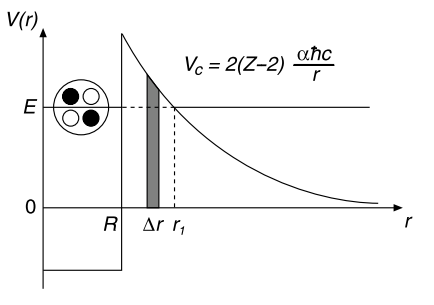
\includegraphics[width=0.4\textwidth]{./potential.png}
	\caption[Potential $\alpha$-Zerfall]{Kernpotential beim $\alpha$-Zerfall - gut zu sehen ist der quasistation"are Zustand des gebildeten He-Kernes \cite{povh}.}    
	\label{fig:potential}
\end{wrapfigure}
erlaubt.
\begin{align}
M(Z,A)>M(Z-4,A-2)+M(4,2).
\end{align}
Daher ist die Energie des emittierten Helium-Kerns f"ur jeden Kern scharf definiert, wobei die kinetische Energie des Teilchens etwas geringer ist, da der Kern durch den R"ucksto"s (Impulserhaltung!) etwas an Energie aufnimmt.\par
Eine gute Beschreibung liefert der Tunneleffekt. Dazu nimmt man an, dass der Kern sich als gebundener Zustand in einem Potentialtopf bewegt, welcher ab dem Kernradius $R$ in ein absto"sendes Coulomb-Potential "ubergeht (siehe Abbildung \ref{fig:potential}). Formt sich ein Helium-Kern innerhalb des Mutterkerns vor, so befindet sich dieser in einem quasi-station"aren Zustand, der nur noch durch das Coulomb-Potential am Verlassen des Mutterkerns gehindert wird. Durch den quantenmechanischen Tunneleffekt wird dies jedoch mit einer geringen Wahrscheinlichkeit erm"oglicht. Der frei werdende Helium-Kern wird dann durch die Coulomb-Absto"sung mit der Energie des quasistation"aren Zustandes minus des R"ucksto"ses "'davongeschossen"'.   

\subsubsection{Die $\beta$-Strahlung}   
Bei Nukliden mit deutlichem Neutronen-, bzw. Protonen"uberschuss zerf"allt ein Neutron ($\beta^{-}$-Zerfall), bzw. ein Proton ($\beta^{+}$-Zerfall) durch die schwache Wechselwirkung in folgenden Kan"alen:
\begin{align}
\beta^{-}: n\rightarrow p+e^{-}+\bar{\nu_{e}}\\
\beta^{+}: p\rightarrow n+e^{+}+\nu_{e}
\end{align}
Dieser Zerfall stellt ein Beweis f"ur die Existenz von Neutrinos dar. Dieses muss am Prozess beteiligt sein, da keine fest definierten Energien der emittierten Elektronen, bzw. Positronen beobachtet wird, sodass zwar eine breite Energieverteilung entsteht, die aber ein charakteristisches Maximum besitzt.\par 
Des Weiteren existiert ein zus"atzlicher Reaktionskanal, der inverse $\beta^{-}$-Zerfall, bei dem ein H"ullenelektron aus der K-Schale mit einem Proton des Kerns zu einem Neutron und einem Elektron-Neutrino reagiert. 


\subsubsection{Die $\gamma$-Strahlung}
Durch die oben genannten Zerfallsarten k"onnen die Tochter-Kerne nach Emission der jeweiligen Teilchen in einem angeregten Zustand mit geringer Lebensdauer verbleiben und durch Aussenden einen Photons mit charakteristischer Energie in einen Zwischen-, bzw. in den Grundzustand "ubergehen. Dabei entstehen verschiedene Arten von elektromagnetischer Multipolstrahlung. Dies bildet die Grundlage der Gamma-Spektroskopie zur Identifizierung verschiedener radioaktiver Materialien, welche auch hier im Praktikumsversuch verwendet wurde. 

\subsubsection{Weitere Strahlungsarten}
Besitzt ein Kern eine relativ zu gro"se Anzahl an Protonen bzw. Neutronen, so k"onnen diese direkt aus dem Kern emittiert werden. Dies geschieht haupts"achlich bei kleinen Kernen wie $^{5}$He nach $^{4}$He oder $^{5}$Li nach $^{4}$Li. \par 
Des Weiteren gibt es spontane Kernspaltung. Nach dem Tr"opfchenmodell der Atomkerne spaltet sich ein Atomkern (anzutreffen bei sehr gro"sen Massenzahlen, $A>270$ \cite{povh}) aufgrund dynamischer Instabilit"at in etwa zwei gleich gro"se Tochterkerne auf, wenn die Coulombabsto"sung des Kerns gr"o"ser wird als die Oberfl"achenspannung. 
Neben dem $\alpha$-Zerfall und der spontanen Spaltung k"onnen auch $^{12}$C-Kerne in einem quasi-station"aren Zustand vorgeformt und emittiert werden. Die Wahrscheinlichkeit daf"ur ist jedoch nur sehr gering, weswegen diese Zerfallsart nur in sehr gro"sen Kernen zu finden ist.  

\subsection{Strahlenschutz}

Wie bereits erw"ahnt, stellt der Umgang mit Radioaktivit"at eine Gefahr f"ur die Gesundheit dar. Durch die ionisierende Wirkung von Strahlung werden Zellen und vor allem das Erbgut in den Zellen besch"adigt. Dies beeintr"achtigt die fehlerfreie Reproduktionsf"ahigkeit und kann zur Ausbildung von Krebs f"uhren, in schlimmen F"allen zu akuter Strahlenkrankheit bis hin zum Tod. Um dies zu vermeiden, sind strikte Strahlenschutzma"snahmen zu treffen. 

\subsubsection{Einheiten im Strahlenmesswesen}
\label{ch:einheiten}
Um Strahlung qualitativ zu erfassen, werden Einheiten zum Rechnen und Vergleichen eingef"uhrt. Die Aktivit"at eines radioaktiven Isotops wird als Anzahl der Kernumwandlungen pro Zeit definiert
\begin{align}
A=\frac{\Delta N}{\Delta t} [\si{\becquerel}=\frac{1}{\si{\second}}],
\end{align}
dabei ist die definierte Einheit Becquerel ($\si{\becquerel}$). Historisch wurde hier die Einheit \textit{Curie} ($1Ci=\SI{37}{\giga\becquerel}$) benutzt.
Die Energiedosis $D$ entspricht der Energie W, die pro Masse $m$ in einem durchstrahlten Stoff deponiert wird. Die Einheit Gray ($\si{\gray}$) wird angegeben als
\begin{align}
D=\frac{\Delta W}{\Delta m} [\SI{1}{\gray}=\frac{\si{\joule}}{\si{\kilogram}}].
\end{align}
Da sich verschiedene Strahlungen bei gleicher Energiedeposition unterschiedlich stark auf biologische Materie auswirken, wird des Weiteren ein Qualit"atsfaktor eingef"uhrt, der die biologische Wirkung der verschiedenen Strahlenarten ber"ucksichtigt. Die "Aquivalentdosis $H$ ergibt sich aus dem Qualit"atsfaktor $Q$ und der Energiedosis $D$
\begin{align}
H=D\cdot Q [\SI{1}{\sievert}=\frac{\si{\joule}}{\si{\kilogram}}].
\end{align} 
Da der Qualit"atsfaktor $Q$ dimensionslos ist, besitzt die Energiedosis $H$ die gleiche SI-Einheiten wie die Energiedosis. Als Einheit wird \textit{Sievert} ($\si{\sievert}$) verwendet. Folgende Werte f"ur $Q$ wurden definiert:
\begin{itemize}
	\item R"ontgen-, Gamma- und Betastrahlung (Q=1)
	\item Neutronenstrahlung (Q=5-20)
	\item Alphastrahlung (Q=20)
\end{itemize}
Daran kann man erkennen, dass Alphastrahlung aufgrund ihres hohen Ionisierungsverm"ogens am gef"ahrlichsten f"ur biologische Materie ist. In diesem Zusammenhang wird eine zus"atzliche Einheit eingef"uhrt, die sich "uber die Ionisierung definiert, die \textit{Ionendosis} $J$. Sie leitet sich "uber die Anzahl der durch Ionisation entstandenen Ladungen pro Masse ab ($[J=\frac{\si{\coulomb}}{\si{\kilogram}}]$). Veraltet wurde hier die Einheit \textit{R"ontgen} [$1R=\SI{2.58}{\cdot10\tothe{-4}\coulomb\per\kilogram}$] benutzt. \par 
Da in der Auswertung dieses Versuchs eine Aufgabe zur Ingestion\footnote{Benutzt wurde hier die angegebene Quelle \cite{vogt-schulz}} (hier: orale Aufnahme von radioaktiven Stoffen) ansteht, wird hier die daf"ur n"otige Formel erl"autert. Die effektive Dosis $E_g$ ergibt sich mit Hilfe eines spezifischen Ingestionskoeffizienten $g_{g,E}$ und der Aktivit"at des aufgenommenen Stoffes $A_g$:
\begin{align}
E_g=g_{g,E}\cdot A_g. \notag
\end{align}
Die Aktivit"atszufuhr $A_g$ des Stoffes setzt sich aus der Aktivit"atskonzentration $a_V$, des pro Tag aufgenommenen Volumens $\dot{V}_g$ und der Aufnahmezeit $t$ zusammen. Es ergibt sich also
\begin{align}
E_g=g_{g,E}\cdot A_g=g_{g,E}\cdot a_V\cdot \dot{V}_g \cdot t.
\label{eq:ingestion}
\end{align} 

\subsubsection{Umweltradioaktivit"at}
\label{ch:umw}
Radioaktive Stoffe sind nicht haupts"achlich von Menschen gemacht. Auch vor dem Atomzeitalter gab und gibt es immer noch nat"urliche Radioaktivit"at in der Natur. Viele nat"urliche schwere Elemente, die urspr"unglich aus Supernova-Explosionen stammen und aus denen unsere Erde teilweise besteht, sind radioaktiv. Da diese gro"steils sehr lange Halbwertszeiten (Zeit, in der eine bestimmte Stoffmenge zur H"alfte zerfallen ist) aufweisen, sind sie auch noch nach 3,5 Milliarden Jahren nachweisbar. Durch ihren Zerfall entstehen viele weitere radioaktive Isotope mit unterschiedlichen Halbwertszeiten. Drei in der Natur vorkommende Zerfallsreihen sind wichtig:
\begin{itemize}
	\item $^{232}_{90}$Th $\Rightarrow ^{208}_{82}$Pb (Thorium-Reihe)
	\item $^{235}_{92}$U $\Rightarrow ^{207}_{82}$Pb (Uran-Actium-Reihe)
	\item $^{238}_{92}$U $\Rightarrow ^{206}_{82}$Pb (Uran-Radium-Reihe)
\end{itemize}
Durch diese Reihen kommen Stoffe wie $^{226}_{88}$Ra in Boden und $^{222}_{86}$Rn in Luft vor. Besonders letzteres kann aus W"anden und B"oden herausdiffundieren und sich in schlecht bel"ufteten (Keller-)R"aumen in gef"ahrlich hohen Konzentrationen ansammeln. \par 
Doch nicht nur durch diese Zerfallsreihen entstehen radioaktive Isotope, auch die kosmische Strahlung produziert in der Atmosph"are fortlaufend vor allem $^{14}_{6}$C (wichtig f"ur Radiocarbon-Datierung zur Altersbestimmung). Das Kalium-Isotop $^{40}_{19}$Ka, welches mit einer Konzentration von 0.0117\% in nat"urlichem Kalium vorkommt, ist als primordiales Nuklid mit einer Halbwertszeit von etwa $\si{10\tothe{9}\year}$ schon bei der Entstehung der Erde vorhanden gewesen. Beide Isotope werden durch den Verzehr von Speisen im K"orper aufgenommen.\par 
Allgemein ist die nat"urliche Strahlenbelastung sehr ortsabh"angig. Zum Beispiel ist der Einfluss von H"ohenstrahlung im Gebirge st"arker als im Flachland und auch die aus dem Erdboden austretende Radioaktivit"at h"angt stark von der geologischen Beschaffenheit ab. So ist beispielsweise die Belastung im Erzgebirge gr"o"ser als im Vogelsberg. Im Mittel erf"ahrt jeder Mensch in Deutschland somit eine Strahlenbelastung von $\SI{2}{\milli\sievert}$ durch nat"urliche Strahlung. \par 
Wie bereits erw"ahnt, gibt es neben der nat"urlichen auch die vom Mensch verursachte Radioaktivit"at in der Umwelt. Gr"o"sere Reaktorunf"alle, wie am Three-Mile-Island-AKW (INES: 5), in Tschernobyl und Fukushima (beide INES: 7)\footnote{INES: Internationale Bewertungsskala f"ur nukleare Ereignisse. Skala von 1 bis 7, wobei 7 als "Katastrophaler Unfall" mit einer Freisetzung von Radioaktivit"at $>$ einigen $\SI{10000}{\tera\becquerel} ^{131}$Iod entspricht.} und die Atombombentests in den 60er Jahren des 19. Jahrhunderts, entlie"sen viele Tonnen radioaktiven Materials ganz unterschiedlicher Zusammensetzung in die Umwelt, was heute noch nachgewiesen werden kann. \par 
Doch auch durch medizinische Anwendungen wie R"ontgen, Szintigrafie, CT und Strahlentherapie wird einiges an Strahlendosis im K"orper deponiert. Im j"ahrlichen Mittel wird "uber k"unstliche Strahlenquellen etwa $\SI{2}{\milli\sievert}$ an Strahlung deponiert. Insgesamt ergibt sich f"ur eine in Deutschland lebende Person also eine j"ahrliche Strahlendosis von etwa $\SI{4}{\milli\sievert}$ \cite{cite4}. 


\subsubsection{Abschirmung von Strahlung}

Aufgrund der unterschiedlichen Eigenschaften der verschiedenen Strahlenarten f"uhren diverse Strategien zum Ziel (Abschirmung). Die Helium-Kerne der $\alpha$-Strahlung zum Beispiel werden schon durch wenige $\si{\centi\meter}$ Luft oder einem Blatt Papier gestoppt. \par 
Einige Meter Luft oder d"unne Aluminium-Platten reichen, um $\beta$-Strahlung abzuwehren. Ein effektiver Absorber besteht aus zwei Teilen, einem Kunststoff, der Energie der Elektronen durch Streuung aufnimmt und einer Bleischicht, um die dabei entstehende elektromagnetische Bremsstrahlung abzuschirmen.
\par 
Allgemein l"asst sich elektromagnetische $\gamma$-Strahlung  nur gut durch Materialien mit hoher Kernladungszahl absorbieren, dabei bietet sich haupts"achlich Blei an. Dies wird ganz offensichtlich auch in der Medizin zur Abschirmung beim R"ontgen benutzt. \par  
Neutronen lassen sich aufgrund ihrer fehlenden Ladung nur recht schwierig abschirmen, hier verwendet man eine Kombination aus verschiedenen Materialien. Zum Abbremsen (Moderation) wird haupts"achlich ein Kunststoff verwendet, da Neutronen nur durch elastische St"o"se Energie verlieren und die Energieabgabe bei zwei gleich gro"sen Sto"spartnern (Protonen im wasserstoffhaltigen Kunststoff) am gr"o"sten ist. In einem zweiten Material m"ussen die nun thermischen (langsamen) Neutronen eingefangen werden. Dabei wandelt man die Kerne des Materials durch Neutronenanreicherung um. Die dabei entstehende Gamma-Strahlung wird mit einem dritten Material (Blei) abgeschirmt. \par 
Anhand dieser Beispiele kann man sich deutlich machen, wie die Q-Faktoren aus Kapitel \ref{ch:einheiten} zustande kommen. Bis jetzt wurde hier nur die Abschirmung von Strahlung au"serhalb des K"orpers behandelt. Wird ein Strahler erst inkorporiert, so liegt eine ernste Gefahr vor. Da $\alpha$-Strahlung auf sehr kurzen Strecken ihre gesamte Energie abgibt, wird die komplette Strahlkraft eines inkorporierten $\alpha$-Strahlers im K"orper deponiert, wohingegen ein Teil der $\beta$- und Gamma-Strahlung den K"orper ohne Wechselwirkung verlassen kann. \par 
Beim Umgang mit radioaktiven Material sollte immer auf die vier A`s des Strahlenschutzes geachtet werden:
\begin{enumerate}
	\item Abstand: so gro"s wir m"oglich. 
	\item Aktivit"at: so gering wie m"oglich/n"otig.
	\item Aufenthaltsdauer: so kurz wie m"oglich/n"otig.
	\item Abschirmung: so gro"s wir m"oglich.
\end{enumerate}
  
\subsection{Detektoren}

Um nun Strahlenschutz oder Forschung zu betreiben, ist es wichtig Strahlung messen zu k"onnen. Da au"ser der Neutronenstrahlung alle Arten von Strahlung eine ionisiernde Wirkung auf Materie haben, kann man sich diesen Effekt zu nutze machen und mit Hilfe verschiedener Detektoren-Typen die Ionisierung indirekt messen. Beim Szintillationsz"ahler wird dabei die Menge der entstehenden Photonen, beim Halbleiterdetektor die Anzahl der entstandenen Elektronen gez"ahlt und so ein R"uckschluss auf die Energie der Teilchen gewonnen. 

\subsubsection{Szintillationsz"ahler}
Ein Szintillator ist ein Material, dessen Atome bzw. Molek"ule beim Durchgang von geladenen Teilchen (oder Photonen) angeregt werden und Photonen emittieren. Die verwendeten anorganischen Szintillatoren haben eine f"ur Kristalle typische Bandstruktur. Ionisierende Strahlung kann aus dem Valenzband freie Elektronen oder  
\begin{wrapfigure}{r}[2cm]{0.4\textwidth}
 	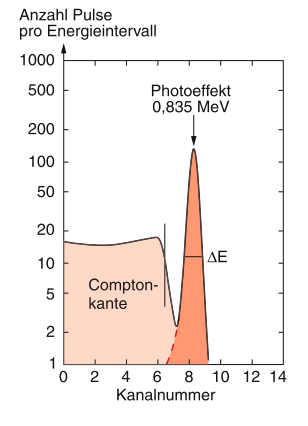
\includegraphics[width=0.4\textwidth]{./szinti.png}
 	\caption[Energiespektrum Szintillator]{Das Energiespektrum eines Szintillationsz"ahlers beim Durchgang monoenergetischer $\gamma$-Strahlung mit einer Energie von $\SI{835}{\kilo\electronvolt}$ \cite{demtroeder}.}    
 	\label{fig:spektrum_szinti}
\end{wrapfigure}
\noindent
Elektron-Loch-Paare erzeugen, welche die eingebrachten Aktivatorzentren anregen k"onnen. Unter Photonenemission fallen diese wieder in ihren Grundzustand zur"uck, wobei die Lichtausbeute durch passendes Dotieren von Aktivatoren (z.B. Tallium) erh"oht werden kann. Dabei sollte beachtet werden, dass das Szintillationsmaterial transparent f"ur die charakteristischen Wellenl"angen des von den Exzitonen emittierten Lichtes ist.
\par 
Die Anzahl der entstehenden Photonen $N_{ph}=\delta \cdot E_{kin}/h\nu$ ist von verschiedenen Faktoren abh"angig. Hierbei sind vor allem die Quantenausbeute $\delta$ des Materials und die Quantenausbeute $\eta$ der Photokathode des Photomultipliers zu nennen. Weiterhin wird die Photonenzahl durch Absorption und unvollst"andige Reflexion an den R"andern des Materials beeinflusst, wodurch Photonen mit dem Faktor $\beta$ verloren gehen. Durch den photoelektrischen Effekt werden dann an der Photokathode $\eta \cdot \beta \cdot N_{ph}$ Elektronen emittiert, die im Photomultiplier vervielfacht werden. Dies geschieht, indem die Elektronen durch ein elektrisches Feld zu hintereinander geschalteten Dynoden beschleunigt werden und an diesen Sekund"arelektronen herausschlagen. Von Dynode zu Dynode nimmt somit der Elektronenstrom zu. Dadurch ergibt sich an der abschlie"senden Anode mit einer Ausgangskapazit"at $C$ ein Spannungspuls von $U=M\cdot \eta \cdot N_{ph} \cdot e/C$. Da die Quantisierungsverluste im Vergleich zum Halbleiterdetektor um einiges gr"o"ser sind, ist die Energieaufl"osung des Szintillationsz"ahlers um einige Gr"o"senordnungen schlechter. Auch Photonen k"onnen mit einem Szintillator nachgewiesen werden. Durch Photo- und Compton-Effekt entstehen Sekund"arelektronen, die dann den oben beschriebenen Effekt im Leitungsband hervorrufen k"onnen. Beim Compton-Effekt entsteht neben dem Compton-Elektron ein weiteres Photon, dass den Detektor entweder verlassen oder wieder durch den Photo-Effekt eingefangen werden kann. Dadurch erh"alt man in der Energieverteilung ein scharfes Maximum bei der eigentlichen Photonenenergie der zu detektierenden Strahlung und ein flacheres, breiteres Spektrum mit niedrigerer Energie, das von den Compton-Elektronen hervorgerufen wird. 
\begin{center}
	\centering
	\begin{figure}[h]
		\centering
		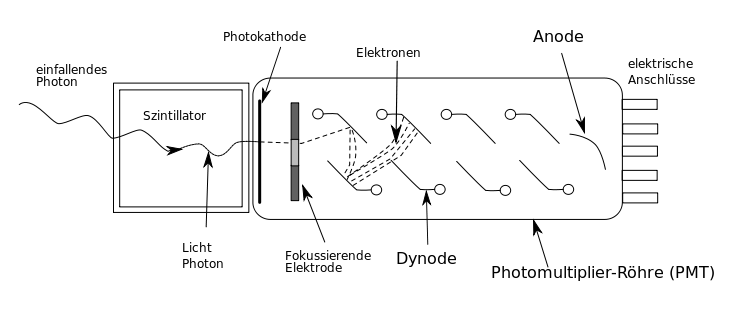
\includegraphics[width = 0.75\linewidth]{./PMT.png}
		\caption[Szintillator]{Aufbau des Photomultipliers mit Szintillator. \newline Bildquelle: \url{http://bit.ly/2fpBmF4} [30.12.2016].}
		\label{fig:PMT}
	\end{figure}
\end{center}

\subsubsection{Halbleiterdetektoren}

Ein Halbleiterdetektor ist ein in Sperrrichtung betriebener p-n-"Ubergang einer Halbleiterdiode. Beim Durchgang eines geladenen Teilchens werden in der Verarmungsschicht viele Elektron-Lochpaare erzeugt, die aufgrund des angelegten elektrischen Feldes an den Elektroden gesammelt werden. Analog zum Gas-Ionisationsdetektor wird die Energie des Teilchens in Form von freien Ladungstr"agern deponiert. Dabei 
erzeugt der Halbleiterdetektor jedoch schneller und um einiges mehr Ladungstr"ger pro Energieverlust $\Delta E$, was zu einer viel sch"arferen Energieaufl"osung f"uhrt. \par 
Als Materialien werden haupts"achlich hochreine Silizium- und Germaniumkristalle benutzt, als Donatoren dienen im n-Teil Phosphor oder Antimon (eine Hauptgruppe h"oher), im p-Teil Bor oder Aluminium (eine Hauptgruppe niedriger). F"ur die "Ubergangszone gilt $d\sim\sqrt{U}$, daher wird Hochspannung U benutzt, um eine m"oglichst gro"se Verarmungszone d zu bekommen. Hier gilt es, einen Durchbruch zu vermeiden, ebenfalls sollte man die Diode keinesfalls in Druchlassrichtung anschlie"sen, da in beiden F"allen der Detektor sofort zerst"ort werden w"urde. \par 
Um das effektive Volumen der Verarmungszone zu vergr"o"sern wird eine intrinsische leicht dotierte n-Schicht zwischen einer sehr stark dotierten p- und n-Schicht eingebracht. Da die Beweglichkeit von Donatoren und Akzeptoren bzw. Gitteratome in einem Festk"orper allgemein von der Temperatur abh"angt, wird der Detektorkristall dauerhaft mit fl"ussigem Stickstoff gek"uhlt, um die thermische Diffusion der stark dotierten Schichten zu vermeiden, die sonst den Detektor sch"adigen w"urden. Dieses Prinzip wurde in der Vergangenheit zum Beispiel in mit Lithium dotierten Germaniumz"ahlern ( Ge(Li) ) verwendet. \par 
Aktuelle Detektoren bestehen jedoch aus hochreinen Germaniumkristallen (HPGe: \textit{High Purity Germanium}), die nicht dauerhaft gek"uhlt werden m"ussen. W"ahrend des Betriebes jedoch wird der Detektorkristall mit fl"ussigem Stickstoff gek"uhlt, um thermisches Rauschen zu reduzieren.     
\begin{figure}
	\centering
	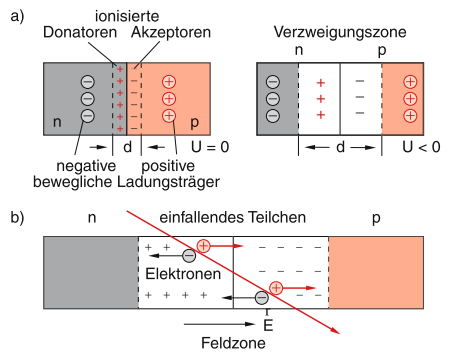
\includegraphics[width=0.6\textwidth]{./hl.png}
	\caption[Halbleiterdetektor]{Der p-n-"Ubergang eines Halbleiterdetektors. a) Entstehung der Verarmungszone. b) Produktion von Elektron-Loch-Paaren beim Durchgang ionisierender Strahlung \cite{demtroeder}.}   
	%\vspace{-110pt} %removes the whitebox on the other page 
	\label{fig:hl}
\end{figure}
\vfill
\clearpage


\section{Versuchsteil 1: Gammaspektroskopie}

In diesem Versuchsteil soll sich mit der Benutzung eines Germanium-Halbleiterdetek\-tors vertraut gemacht werden, indem einige $\gamma$-Spektren aufgenommen werden. Dazu geh"ort die Aufnahme einiger charakteristischer Spektren von radioaktiven Proben, eine Langzeitaufnahme des radioaktiven Untergrundes der Praktikumsr"aumlichkeiten, sowie die Untersuchung eines Haushaltsgegenstandes. Die Proben wurden dabei direkt vor dem Detektor positioniert (siehe Abb. \ref{fig:schaltbild}).
\begin{figure}[h]
	\centering
	\makebox[\textwidth]{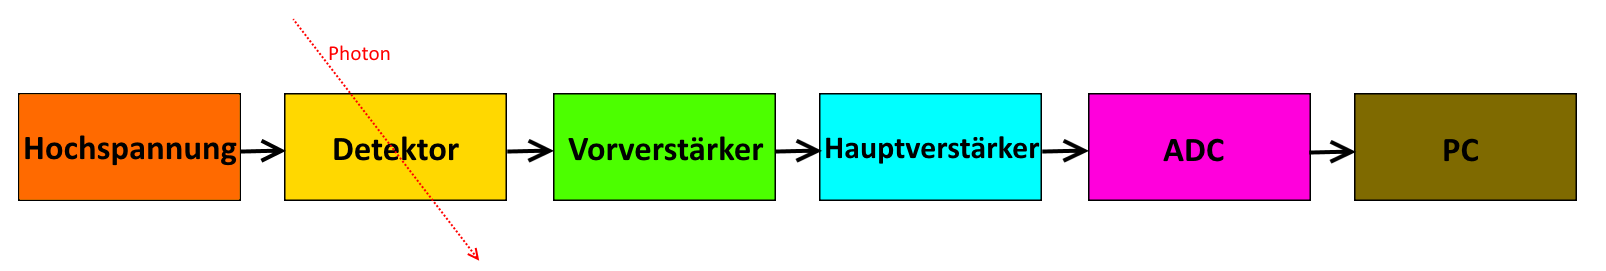
\includegraphics[width=0.85\paperwidth]{./blockschaltbild.png}}
	\caption[Blockschaltbild]{Blockschaltbild des Detektor-Aufbaus. Die Hochspannung versorgt den Detektor, das analoge Rohsignal wird "uber einen Vorverst"arker und einen Hauptverst"arker mit Hilfe eines AD-Wandlers digitalisiert und zur Datenaufnahme in einen PC geleitet.} \label{fig:schaltbild}
\end{figure}
    

\subsection{Energieeichung}

Um nun den Kan"alen des AD-Wandlers geeignete Energiewerte zuordnen zu k"onnen, wurde eine Eichung mit Hilfe bekannter Strahler durchgef"uhrt. Das Spektrum ist in Abbildung \ref{fig:eichspektrum} zu finden. In Tabelle \ref{tab:eichung_roh} findet man die mit der Software \textit{MCA} am Arbeitsplatz gefitteten Werte der Energieeichung.  
\begin{table}[b!]
	\centering
	\small
	\begin{tabular}{cccc}
		\hline 
		\rowcolor[gray]{0.8} Nuklid & $E_{\gamma} [\si{\mega\electronvolt}]$ & Kanal K & Fehler $\Delta K$ (Gau"s-Fit) \\ 
		\hline 
		Cs137 & 0.6617 & 1582.46 & 0.0122403 \\ 
		\hline 
	\rowcolor[gray]{0.95}	Co60 & 1.17324 & 2809.28 & 0.0160256 \\ 
		\hline 
		& 1.3325 & 3191.38 & 0.0227815 \\ 
		\hline 
	\rowcolor[gray]{0.95} Na22	& 0.510999* & 1220.84 & 0.0288171 \\ 
		\hline 
		& 1.2746 & 3052.26 & 0.0252888 \\ 
		\hline 
	\rowcolor[gray]{0.95} Bi207	& 0.5697 & 1361.83 & 0.0101928 \\ 
		\hline 
		& 1.0637 & 2546.66 & 0.0149209 \\ 
		\hline 
	\rowcolor[gray]{0.95} Ba133	& 0.0810 & 188.742 & 0.0396785 \\ 
		\hline 
		& 0.2764 & 657.938 & 0.0177448 \\ 
		\hline
	\rowcolor[gray]{0.95}	& 0.3029 & 721.457 & 0.0126372 \\ 
		\hline 
		& 0.3560 & 849.036 & 0.0138227 \\ 
		\hline
	\rowcolor[gray]{0.95}	& 0.3839 & 915.836 & 0.0130588 \\ 
		\hline 
		& 0.4370 & 1043.18 & 0.0354023 \\ 
		\hline
	\end{tabular} 
	\caption{Werte der Energieeichung. Die Energien zur Eichung $E_{\gamma}$ wurden aus \cite{cite1} "ubernommen. Der Kanal wurde mit einem Gau"s-Fit bestimmt. *Die Energie der Photonen aus der $e^{-}e^{+}$-Annihilation kommt aus \cite{cite2}.}
	\label{tab:eichung_roh}
\end{table}

\begin{figure}[h!]
	\centering
	\includegraphics[width=1\linewidth]{./20161216/eichspektrum.png}
	\caption[Eichspektrum]{Eichspektren der verschiedenen benutzten Quellen. **Im vergr"o"serten Ausschnitt sind zwei Peak-Gruppen des $^{207}$Bi um den $\SI{81}{\kilo\electronvolt}$-"Ubergang des $^{133}$Ba verteilt. }
	\label{fig:eichspektrum}
\end{figure}
\noindent
Mit Hilfe von \textit{OriginPro 9.3} wurde gem"a"s Anleitung \cite{cite1} ein linearer Fit mit 
\begin{align}
K(E)&=m\cdot (E-E_{0})+b
\intertext{durchgef"uhrt. Dabei wurden die Energien auf den mit den quadratisch gewichteten Fehlern berechneten Schwerpunkt $E_{0}$ verschoben, um Kovarianzen zwischen $\Delta$m und $\Delta$b zu vermeiden (nach \cite{cite3}, Kap. 1.3). F"ur $E_{0}$ gilt also}
E_{0}&=\frac{\sum_{i}\frac{1}{(\Delta K_{i})^{2}}E_{i}}{\sum_{i}\frac{1}{(\Delta K_{i})^{2}}}=\SI{0.61755}{\mega\electronvolt} 
\intertext{und der Fit liefert}
m&=(2398.8265\pm 0.14063)\frac{1}{\si{\mega\electronvolt}} \notag \\
b&=1476.39668\pm 0.04678. \notag
\end{align}
Der Fehler des Fits wurde mit der reduzierten Fehlerquadratsumme $\chi^{2}$ multipliziert. Um die G"ute des Fits zu "uberpr"ufen und um m"ogliche Eingabefehler auszuschlie"sen, wurden neben dem Plot der Eichgeraden auch die Residuen gezeichnet (Abb. \ref{fig:eichung}). 
\begin{figure}
	\centering
	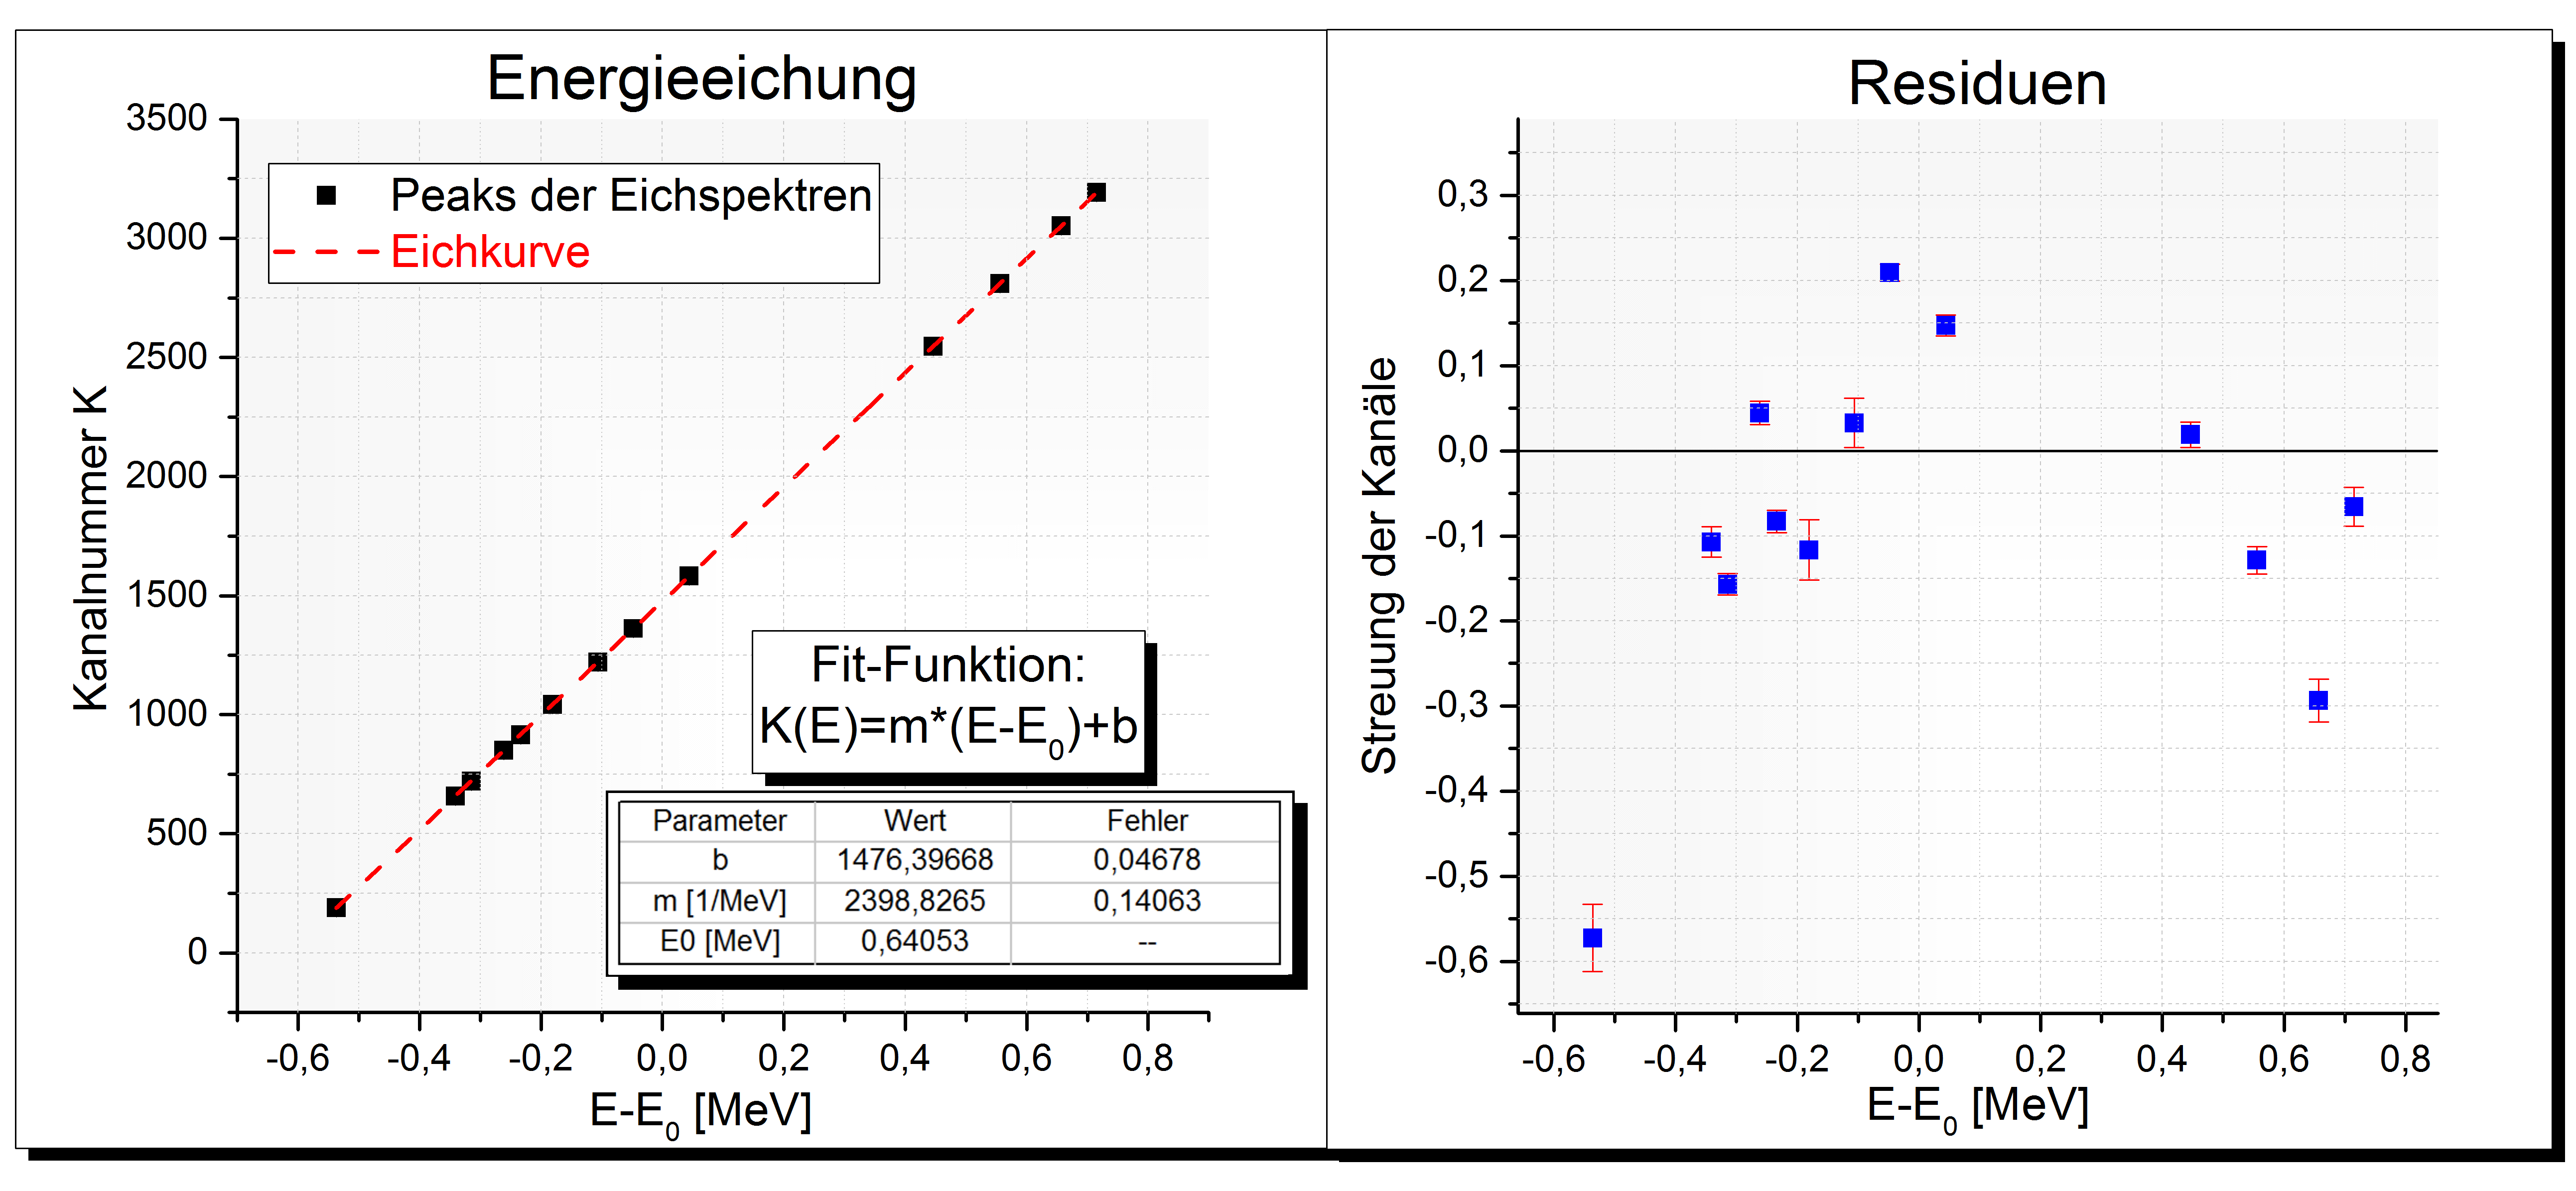
\includegraphics[width=\linewidth]{./20161216/energieeichung2.png}
	\caption[Energieeichung und Residuen]{Energieeichung und Residuen. Die Energien wurden aus \cite{cite1} "ubernommen. }
	\label{fig:eichung}
\end{figure}
Die Residuen streuen im Mittel um etwa $0.15$ Kan"ale um die Eichgerade, wobei der "Ubergang von $^{133}Ba: E_{\gamma}=\SI{0.0810}{\mega\electronvolt}$ im sehr niedrigen Kanal $K\approx 189$ st"arker abweicht. Dies resultiert aus der in diesem Kanalbereich nicht mehr linearen Verst"arkung. Mit Hilfe der Eichfunktion K(E-$E_{0}$) kann nun die Kanalzahl durch Umstellen in die entsprechende Energie umgewandelt werden:
\begin{align}
E(K)=\frac{K-b}{m}+E_{0} 
\label{eq:energie}
\end{align} 
Mit Hilfe der Gau"sschen Fehlerfortpflanzung kann man den Fehler f"ur die Energie in \eqref{eq:energie} berechnen:
\begin{align}
\Delta E&=\sqrt{\left(\frac{\partial E}{\partial m}\Delta m\right)^{2}+\left(\frac{\partial E}{\partial b}\Delta b\right)^{2}+\left(\frac{\partial E}{\partial K}\Delta K\right)^{2}} \notag\\
&=\sqrt{\left(\frac{b-K}{m^{2}}\Delta m\right)^{2}+\left(-\frac{1}{m}\Delta b\right)^{2}+\left(\frac{1}{m}\Delta K\right)^{2}}
\label{eq:fehler}
\end{align} 
Das R"uckrechnen der Werte mit entsprechenden Fehlern liefert Tabelle \ref{tab:rueck}. Man erkennt, dass die Abweichungen f"ur die Werte mit den gr"o"sten Residuen am gr"o"sten werden(K$\approx$3052 und Kanal K$\approx$189). Ohne Ber"ucksichtigung dieser Werte liegen vier von elf Werte innerhalb des Fehlers, dies entspricht einer Rate von etwa 36\%. Nimmt man den Fehler als doppelt so gro"s an, also $\Delta E=2\cdot \Delta E_{z}$, so liegen acht von elf Werten innerhalb des Fehlers mit einer Rate von etwa 72\%. Dies w"urde eine Sicherheit von 1$\sigma$ ergeben. Mit Hilfe der Eichung wurden die Eichspektren gegen die Energie aufgetragen, zu finden in Abbildung \ref{fig:eichspektrum}. 
\begin{table}[h!]
	\centering
	\small
	\makebox[\textwidth]{
	\begin{tabular}{cccccc}
		\hline 
		\rowcolor[gray]{0.8} Kanal K & Fehler $\Delta$K & \pbox{5cm}{Energie $E_{Lit}$ \\ $[\si{\mega\electronvolt}]$  } & \pbox{5cm}{Energie $E_{z}$ \\ $[\si{\mega\electronvolt}]$  } & \pbox{5cm}{Fehler \\ $\Delta E_{z} [10^{-5}\si{\mega\electronvolt}]$} & \pbox{6cm}{Abweichung \\ $|E-E_{z}| [10^{-5}\si{\mega\electronvolt}]$}\\ 
		\hline 
		3191.38 & 0.0227815 & 1.3325 & 1.33247 & 4.71922 &  0.27387 \\ 
		\hline 
	\rowcolor[gray]{0.95}	3052.26 & 0.0252888 & 1.2746 & 1.27448 & 4.44369 &  12.24116 \\ 
		\hline 
		2809.28 & 0.0160256 & 1.17324 & 1.17319
		 & 3.85490 & 5.36045  \\ 
		\hline 
	\rowcolor[gray]{0.95}	2546.66 & 0.0149209 & 1.0637 & 1.06371 & 3.32132 &  0.78653  \\ 
		\hline 
		1582.46 & 0.0122403 & 0.6617 & 0.66176
		 & 2.03236 & 6.13304  \\ 
		\hline 
	\rowcolor[gray]{0.95}	1361.83 & 0.0101928 & 0.5697 & 0.56978 & 2.01539 & 8.71921   \\ 
		\hline 
		1220.84 & 0.0288171 & 0.510999 & 0.511013 & 2.37412 & 0.78651   \\ 
		\hline 
	\rowcolor[gray]{0.95}	1043.18 & 0.0354023 & 0.4370 & 0.43695 & 2.66489 &  4.85932  \\ 
		\hline 
		915.836 & 0.0130588 & 0.3839 & 0.38386 & 2.44461 &  3.45491 \\ 
		\hline 
	\rowcolor[gray]{0.95}	849.036 & 0.0138227 & 0.3560 & 0.35602 & 2.54668 & 1.85014  \\ 
		\hline 
		721.457 & 0.0126372 & 0.3029 & 0.30283 & 2.73580 & 6.54201  \\ 
		\hline
	\rowcolor[gray]{0.95}	657.938 & 0.0177448 & 0.2764 & 0.27636 & 2.88976 &  4.46175  \\ 
		\hline
		188.742 & 0.0396785 & 0.0810 & 0.08076 & 4.05487 & 23.85881   \\ 
		\hline 
	\end{tabular} }
	\caption{R"uckrechnen der Energiewerte mit Hilfe der Energieeichung. Dabei ist $E_{Lit}$ der Literaturwert und $E_{z}$ der zur"uckgerechnete Wert.}
	\label{tab:rueck}
\end{table}
\noindent
Auff"allig im $^{207}$Bi-Spektrum sind einige sehr ereignisreiche Peaks im niedrigen Energiebereich (in Abb. \ref{fig:eichspektrum} mit ** markiert).  
\begin{wraptable}{r}{0.35\linewidth}
	\centering
	\small
	\begin{tabular}{cc}
			\hline
			\rowcolor[rgb]{ .749,  .749,  .749} Energie [keV] & Ursprung \\
			\hline
			72.8042 & K$_{\alpha 2}$ \\
			\hline
			\rowcolor[rgb]{ .949,  .949,  .949} 74.9694 & K$_{\alpha 1}$ \\
			\hline
			84.9  & K$_\beta$ \\
			\hline
			\rowcolor[rgb]{ .949,  .949,  .949} 74.8148 & K$_{\alpha 2}$ \\
			\hline
			77.11 & K$_{\alpha 1}$ \\
			\hline
			\rowcolor[rgb]{ .949,  .949,  .949} 87.3  & K$_{\beta}$ \\
			\hline
	\end{tabular}%
	\label{tab:xray}%
	\caption{\small Die Daten f"ur die Anregungsenergie der Atomh"ulle von $^{207}$Bi wurden "ubernommen aus \cite{IAEA}.}
	\vspace{-100pt} %removes the whitebox on the other page 
\end{wraptable}
Da diese Energien sich nicht mit Hilfe des Niveauschemas der Anleitung \cite{cite1} erkl"aren lassen, wurde in der Datenbank der IAEA\footnote{International Atomic Energy Agency} \cite{IAEA} nachgeschlagen (siehe Tabelle \ref{tab:xray}). Es wurden also in guter "Ubereinstimmung mit den Messwerten Schalenanregungen des Bismut-Atoms gemessen, dabei wird sogar die Feinstrukturaufspaltung der $\alpha$-Linie sichtbar.

\newpage
\subsection{Untergrundspektrum}

Das Untergrundspektrum des Praktikumsraumes wurde insgesamt f"ur t$=\SI{234961}{\second}\approx\SI{65.3}{\hour}$ aufgenommen. In Tabelle \ref{tab:untergrund} sind die deutlichsten Peaks des Untergrundes eingetragen und wie im vorherigen Teil die Energien mit Hilfe der Eichung \eqref{eq:energie} und der Fehlerrechnung \eqref{eq:fehler} umgerechnet. In Plot \ref{fig:untergrund} ist der Untergrund (gr"un) im Vergleich zum Gl"uhstrumpf (blau) gezeichnet.   
% Table generated by Excel2LaTeX from sheet 'untergrund' lol wie es einfach funktioniert, erstaunlich :O
\begin{table}[h!]
	\centering
	\small
	\makebox[\textwidth]{
		\begin{tabular}{cccccccc}
			\rowcolor[rgb]{ .749,  .749,  .749} Kanal K & Fehler dK & \pbox{5cm}{Energie $E_{z}$ \\ $[\si{\kilo\electronvolt}]$  } & \pbox{5cm}{Fehler $E_{z}$ \\ $[\si{\kilo\electronvolt}]$  } & Nuklid & \pbox{5cm}{Energie $E_{Lit}$ \\ $[\si{\kilo\electronvolt}]$  }  & Abweichung [keV] & Nat. Zerfallsreihe \\
			3500.05 & 0.02514 & 1461.14803 & 0.05418 & 40K   & 1460.80000 & 0.34803 & / \\
			\rowcolor[rgb]{ .949,  .949,  .949} 2965.72 & 0.07008 & 1238.40162 & 0.05058 & 214Bi & 1238.10000 & 0.30162 & Uran-Radium \\
			2682.89 & 0.02100 & 1120.49813 & 0.03642 & 214Bi & 1120.30000 & 0.19813 & Uran-Radium \\
			\rowcolor[rgb]{ .949,  .949,  .949} 2547.08 & 0.02502 & 1063.88295 & 0.03426 & 207Bi & 1063.71000 & 0.17295 & / \\
			2309.76 & 0.05494 & 964.95124 & 0.03633 & 228Ac & 964.60000 & 0.35124 & Thorium-Reihe \\
			\rowcolor[rgb]{ .949,  .949,  .949} 2319.88 & 0.02388 & 969.16997 & 0.03007 & 228Ac & 969.11000 & 0.05997 & Thorium-Reihe \\
			2181.26 & 0.01268 & 911.38338 & 0.02655 & 228Ac & 911.07000 & 0.31338 & Thorium-Reihe \\
			\rowcolor[rgb]{ .949,  .949,  .949} 1457.06 & 0.01683 & 609.48577 & 0.02073 & 214Bi & 609.31000 & 0.17577 & Uran-Radium \\
			1394.38 & 0.01215 & 583.35633 & 0.02025 & 208Tl & 583.14000 & 0.21633 & Thorium-Reihe \\
			\rowcolor[rgb]{ .949,  .949,  .949} 1362.12 & 0.02241 & 569.90808 & 0.02180 & 207Bi & 569.70000 & 0.20808 & / \\
			1220.71 & 0.04509 & 510.95843 & 0.02780 & 208Tl & 510.84000 & 0.11843 & Thorium-Reihe \\
			\rowcolor[rgb]{ .949,  .949,  .949} 839.38 & 0.01293 & 351.99403 & 0.02553 & 214Pb & 351.92000 & 0.07403 & Uran-Radium \\
			806.74 & 0.01630 & 338.38488 & 0.02635 & 228Ac & 338.32000 & 0.06488 & Thorium-Reihe \\
			\rowcolor[rgb]{ .949,  .949,  .949} 703.26 & 0.00992 & 295.24920 & 0.02747 & 214Pb & 295.21000 & 0.03920 & Uran-Radium \\
			567.39 & 0.10000 & 238.61026 & 0.05110 & 212Pb & 238.63000 & 0.01974 & Thorium-Reihe \\
			\rowcolor[rgb]{ .949,  .949,  .949} 567.36 & 0.00917 & 238.59484 & 0.02981 & 212Pb & 238.63000 & 0.03516 & Thorium-Reihe \\
			440.75 & 0.11326 & 185.81528 & 0.05701 & 226Ra & 186.21000 & 0.39472 & Uran-Radium \\
		\end{tabular}%
	}
	\caption{Die Peaks der deutlichsten Eintr"age im Untergrundspektrum. Die haupts"achlich gemessenen Energien stammen aus Zerf"allen der nat"urlichen Zerfallsreihen. Die Literaturwerte stammen aus \cite{cite1}.}
	\label{tab:untergrund}
\end{table}%
\noindent
Insgesamt f"allt auf, das zwei Zerfallsreihen, die Uran-Radium- und die Thorium-Zerfallsreihe prominent vertreten sind. Wie in \ref{ch:umw} erw"ahnt, kommen einige nat"urliche radioaktive Stoffe in der Umwelt vor, die auch in geringen Mengen in verbautem Beton oder allgemein im Erdboden vorliegen. Au"serdem findet man in beiden Zerfallsreihen zwei radioaktive Isotope des gasf"ormigen Radons, n"amlich $^{226}$Rn und $^{224}$Rn. Dies ist insgesamt plausibel.\par 
Des Weiteren findet man zwei Elemente, die nicht aus einer nat"urlichen Zerfallsreihe stammen. Die nat"urliche $^{40}$K-Produktion wurde bereits in \ref{ch:umw} erkl"art. Das $^{207}$Bi wurde f"ur die Eichung verwendet und w"ahrend der Messung in einem Tresor verwahrt, bzw. in kleiner Entfernung zum Messstand abgelegt. Da laut Betreuer diese Bismut-Quelle die st"arkste der verwendeten Quellen ist, ist die Abschirmung scheinbar nicht gro"s genug, sodass man einen nicht verschwindenden Eintrag im Spektrum sehen kann.  \par 
Insgesamt sind wieder viele Werte nicht innerhalb des errechneten Fehlers. Dies l"asst sich vermutlich auf wechselnde Umwelteinfl"usse w"ahrend der Messzeit zur"uck\-f"uhren, wie zum Beispiel Temperatur- und Luftdruckschwankungen.  
\begin{figure}[h!]
	\centering
	\makebox[\textwidth]{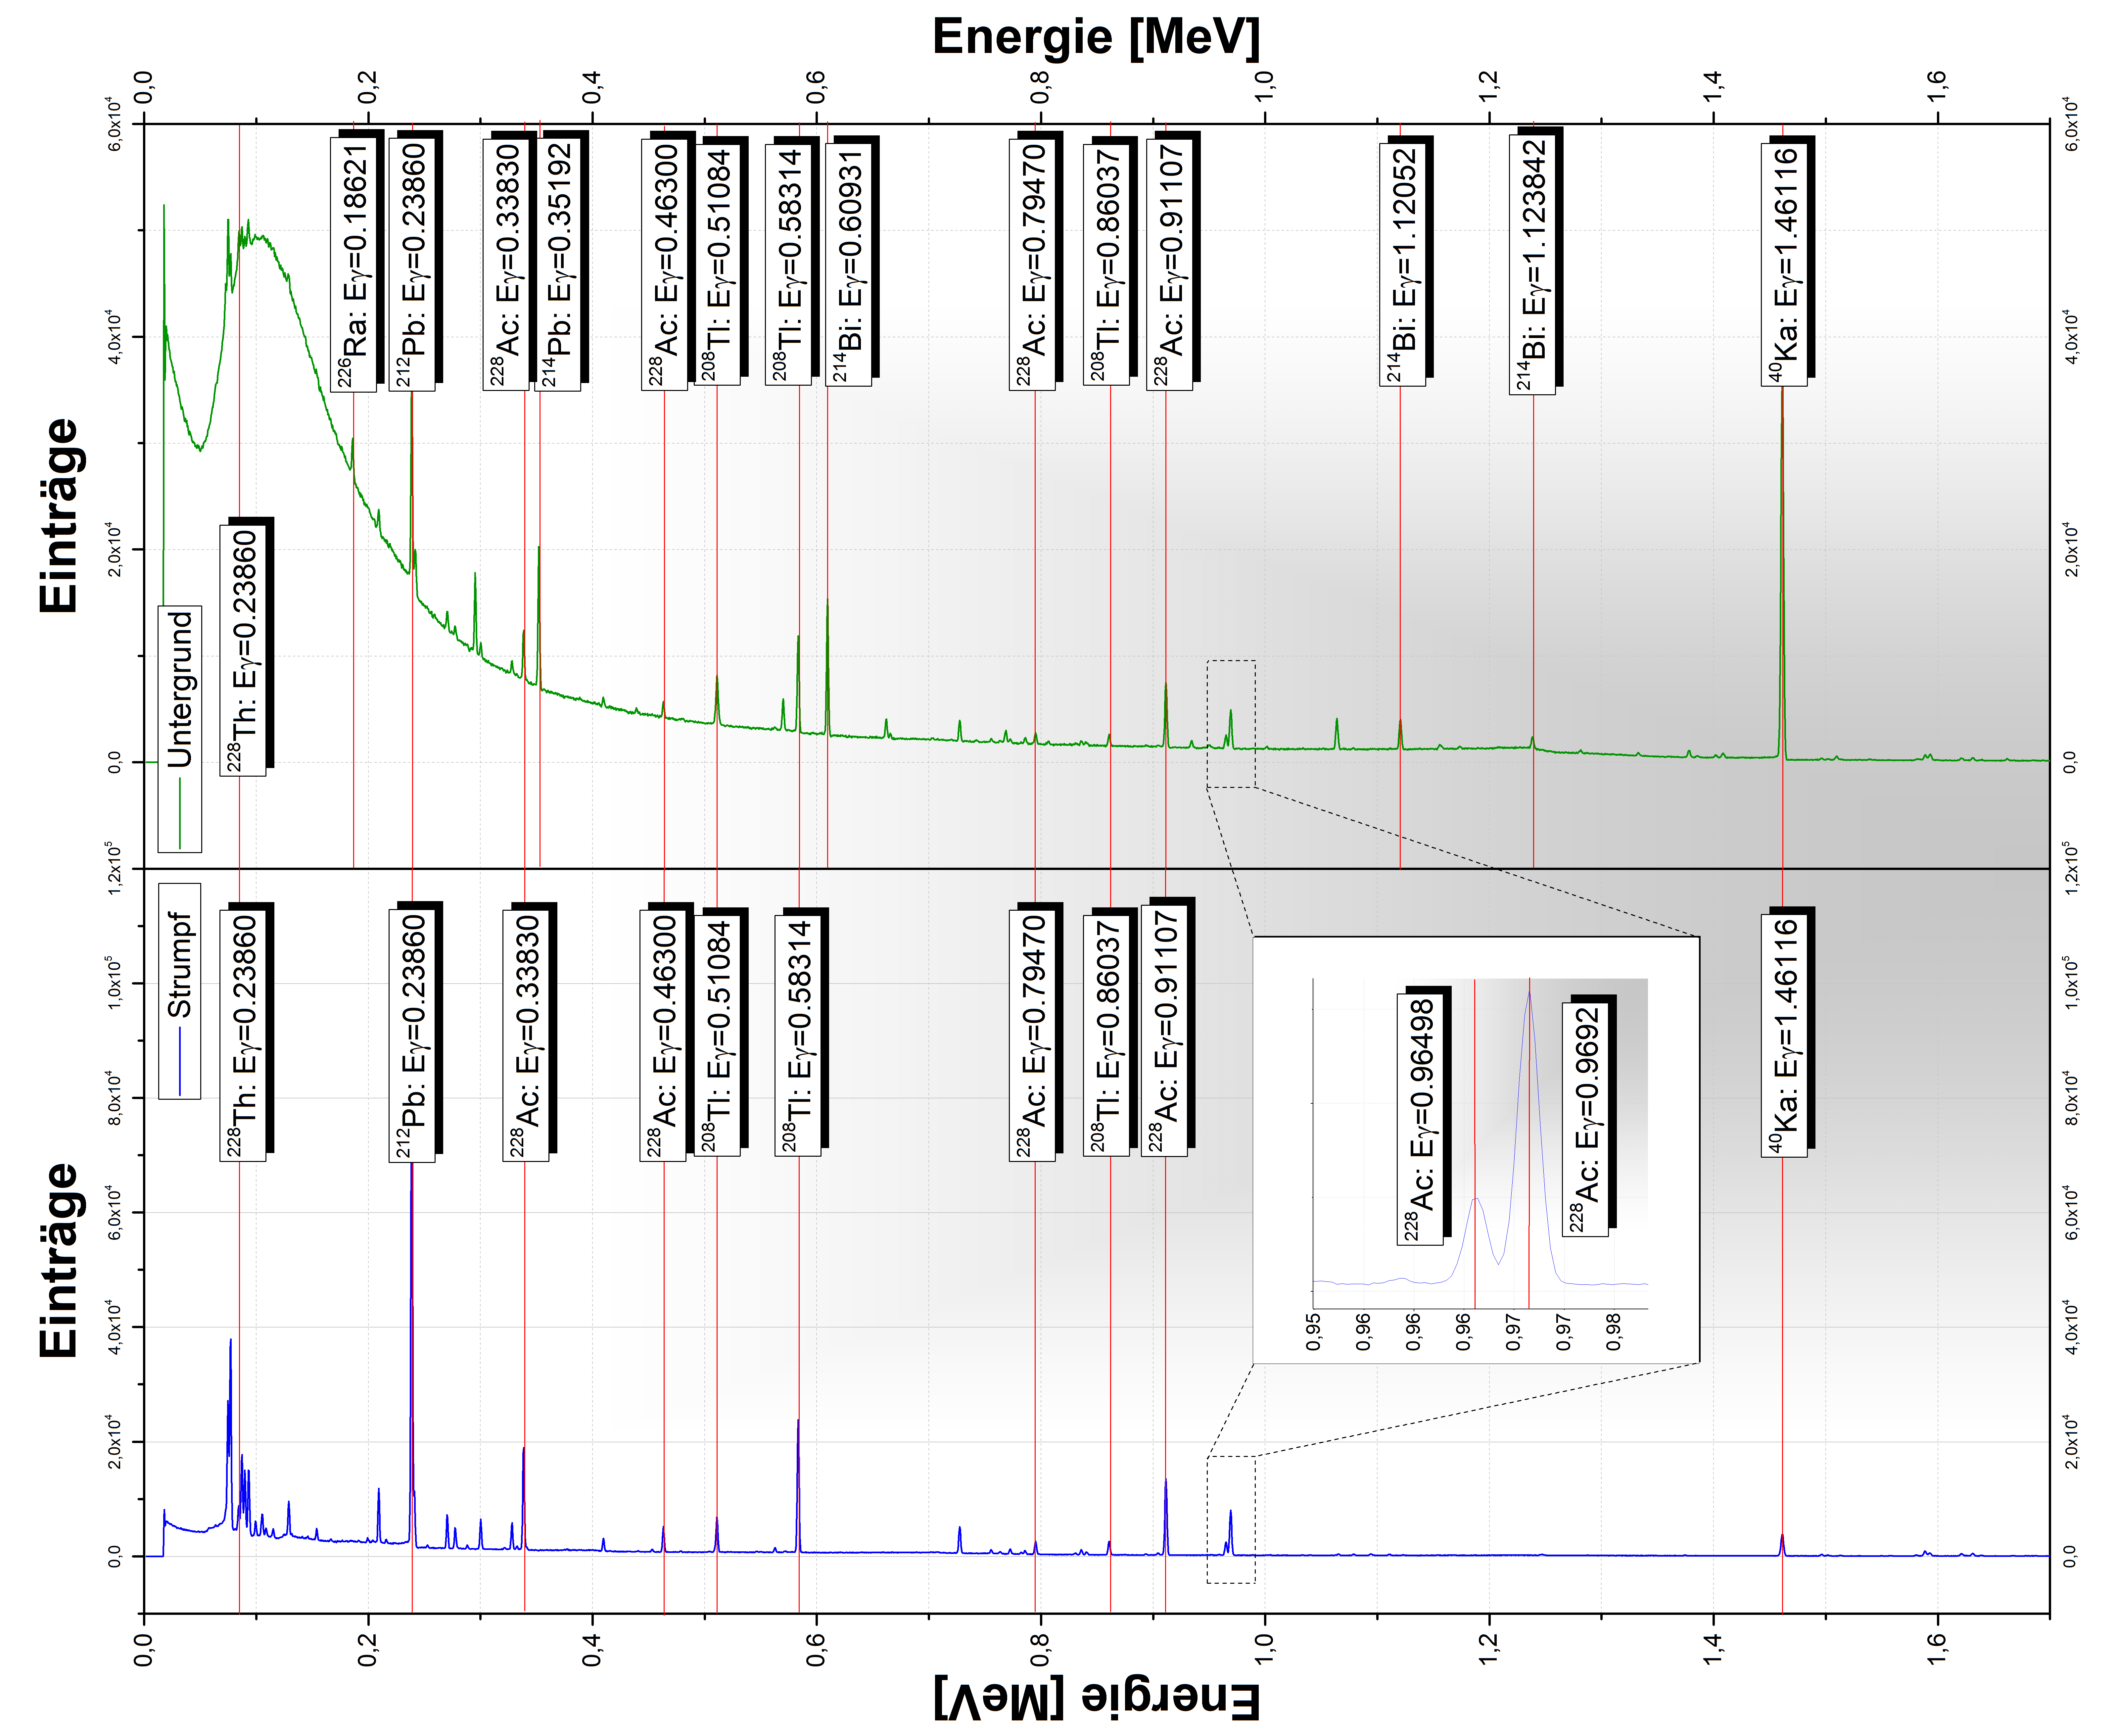
\includegraphics[width=1.1\linewidth]{./20161216/untergrund_strumpf.png}}
	\caption[Untergrund und Gl"uhstumpf]{Untergrund (rechts) und Gl"uhstrumpf (links). Vom Spektrum des Gl"uhstrumpfes wurde der auf die Messdauer von $\SI{6237}{\second}$ normierte Untergrund abgezogen.}
	\label{fig:untergrund}
\end{figure}
\clearpage

\subsection{Haushaltsgegenstand}

Als radioaktiver Haushaltsgegenstand wurde ein Gl"uhstrumpf\footnote{Feinmaschiges Gewebe aus verschiedenen Salzen (unter anderem Thoriumnitrat), dass bei Anregung, z.B. durch die Flamme eines Gaskochers, zum Leuchten gebracht wird.} verwendet. Das Spektrum wurde f"ur insgesamt
t$=\SI{6237}{\second}\approx\SI{1.7}{\hour}$ aufgenommen. In Tabelle \ref{tab:untergrund} sind die deutlichsten Peaks des Untergrundes eingetragen und wie im vorherigen Teil die Energien mit Hilfe der Eichung \eqref{eq:energie} und der Fehlerrechnung \eqref{eq:fehler} umgerechnet. 
\begin{table}[h!]
	\centering
	\small
	\makebox[\textwidth]{
		\begin{tabular}{cccccccc}
			\rowcolor[rgb]{ .749,  .749,  .749} Kanal K & Fehler dK & \pbox{5cm}{Energie $E_{z}$ \\ $[\si{\kilo\electronvolt}]$  } & \pbox{5cm}{Fehler $E_{z}$ \\ $[\si{\kilo\electronvolt}]$  } & Nuklid & \pbox{5cm}{Energie $E_{Lit}$ \\ $[\si{\kilo\electronvolt}]$  }  & Abweichung [keV] & Nat. Zerfallsreihe \\
			\rowcolor[rgb]{ .949,  .949,  .949} 3500.06 & 0.03162 & 1461.15220 & 0.05477 & 40K   & 1460.80000 & 0.35220 & / \\
			2319.72 & 0.02058 & 969.10327 & 0.02964 & 228 Ac & 969.11000 & 0.00673 & Thorium-Reihe \\
			\rowcolor[rgb]{ .949,  .949,  .949} 2309.76 & 0.04326 & 964.95124 & 0.03347 & 228 Ac & 964.60000 & 0.35124 & Thorium-Reihe \\
			2181.14 & 0.00920 & 911.33336 & 0.02630 & 228 Ac & 911.07000 & 0.26336 & Thorium-Reihe \\
			\rowcolor[rgb]{ .949,  .949,  .949} 2059.68 & 0.01398 & 860.70027 & 0.02485 & 208 Tl & 860.37000 & 0.33027 & Thorium-Reihe \\
			1902.28 & 0.02746 & 795.08485 & 0.02489 & 228 Ac & 794.70000 & 0.38485 & Thorium-Reihe \\
			\rowcolor[rgb]{ .949,  .949,  .949} 1739.95 & 0.01215 & 727.41426 & 0.02115 & 212 Bi & 727.17000 & 0.24426 & Thorium-Reihe \\
			1394.30 & 0.01011 & 583.32298 & 0.02005 & 208 Tl & 583.14000 & 0.18298 & Thorium-Reihe \\
			\rowcolor[rgb]{ .949,  .949,  .949} 1220.37 & 0.05060 & 510.81669 & 0.02940 & 208 Tl & 510.84000 & 0.02331 & Thorium-Reihe \\
			1105.94 & 0.01064 & 463.11420 & 0.02195 & 228 Ac & 463.00000 & 0.11420 & Thorium-Reihe \\
			\rowcolor[rgb]{ .949,  .949,  .949} 806.67 & 0.02918 & 338.35903 & 0.02822 & 228 Ac & 338.32000 & 0.03903 & Thorium-Reihe \\
			781.88 & 0.01438 & 328.02190 & 0.02654 & 212 Bi & 327.96000 & 0.06190 & Thorium-Reihe \\
			\rowcolor[rgb]{ .949,  .949,  .949} 660.44 & 0.03182 & 277.39714 & 0.03089 & 208 Tl & 277.35000 & 0.04714 & Thorium-Reihe \\
			643.24 & 0.02129 & 270.22739 & 0.02956 & 228 Ac & 270.23000 & 0.00261 & Thorium-Reihe \\
			\rowcolor[rgb]{ .949,  .949,  .949} 567.33 & 0.02978 & 238.58191 & 0.03206 & 212 Pb & 238.63000 & 0.04809 & Thorium-Reihe \\
			496.80 & 0.01051 & 209.18004 & 0.03119 & 228 Ac & 209.28000 & 0.09996 & Thorium-Reihe \\
			\rowcolor[rgb]{ .949,  .949,  .949} 203.76 & 0.01154 & 87.02197 & 0.03702 & 212 Pb & 87.30000 & 0.27803 & Thorium-Reihe \\
			197.17 & 0.02881 & 84.27271 & 0.03875 & 228 Th & 84.37100 & 0.09829 & Thorium-Reihe \\
			\rowcolor[rgb]{ .949,  .949,  .949} 179.66 & 0.05922 & 76.97539 & 0.04466 & 212,214 Pb & 77.10800 & 0.13261 & Thorium-Reihe \\
			174.17 & 0.08523 & 74.68511 & 0.05153 & 212,214 Pb & 74.81500 & 0.12989 & Thorium-Reihe \\
		\end{tabular}%
	}
	\caption{Peaks der deutlichsten Energien im Gl"uhstrumpf. Alle stammen aus der Thorium-Zerfallsreihe. Der Kalium-Wert resultiert von der "'Probenhalterung"' aus Kaliumchlorid, die auch zur Eichung diente.}
	\label{tab:addlabel}%
\end{table}%
\noindent
Wie zu erwarten findet man nach dem Abzug der Untergrundereignisse nur noch Zerf"alle aus der Thorium-Reihe. Da der Kaliumchlorid-Beh"alter aus der Energieeichung den Gl"uhstrumpf vor den Detektor geklemmt hat, findet man au"serdem noch einen Eintrag f"ur $^{40}$K, der nat"urlich nicht von dem Gl"uhstrumpf kommt.

\subsection{Fragestellungen}

\subsubsection{Strahlenbelastung eines Menschen}
Die Strahlenbelastung eine Menschen w"ahrend eines Fluges in $\SI{10.000}{\meter}$ H"ohe betr"agt etwa D$\approx\SI{5}{\micro\sievert\per\hour}$ \cite{flug1}. Insgesamt h"angt die Strahlendosis von Flugdauer, Flugh"ohe, Dauer des Steig- und Sinkfluges, Flugroute (Breitengrad) und Sonnenaktivit"at ab \cite{flug2}. \par 
F"ur die durch die Kosmische H"ohenstrahlung verursachte effektive Jahresdosis wird in \cite{cite4} etwa D$\approx\SI{1.85}{\milli\sievert\per\year}$ angegeben. Dies bezieht sich auf eine H"ohe von ungef"ahr $\SI{3000}{\meter}$ (Zugspitze). Ebenfalls wird dort eine Effektive Jahresdosis von D$=\SI{0.42}{\milli\sievert\per\year}$ an terrestrischer Strahlung angegeben. Ber"ucksichtigt man diese beiden Werte, so erh"alt man f"ur die Alpen eine effektive Dosis von D$\approx\SI{0.26}{\micro\sievert\per\hour}$.  \par 
An der Meeresk"uste ist der Effekt durch Kosmischen Strahlung geringer, etwa D$=\SI{0.3}{\milli\sievert\per\year}$ \cite{cite4}. Auch hier ist die terrestrische Strahlung sehr ortsabh"angig, so betr"agt sie in Niedersachsen beispielsweise D$=\SI{0.29}{\milli\sievert\per\year}$, woraus sich eine gesamte effektive Dosis von D$\approx\SI{0.06}{\micro\sievert\per\hour}$ ergibt. 

\subsubsection{Reichweite von $\beta$- und $\gamma$-Strahlung in Materie}
Zum Bestimmen der Reichweite von Betastrahlung in Materie wurde die ESTAR-Datenbank des NIST bem"uht \cite{NIST}. Die Berechnungen basieren dabei auf der \textit{continous slowing down approximation} von Elektronen in den jeweiligen Materialien. Mit Hilfe dieser \textit{CSDA-Range} und der Dichte kann man die Reichweite bestimmen:
\begin{align}
R=\frac{R_{CSDA}}{\rho}
\end{align} 
Die Ergebnisse findet man in Tabelle \ref{tab:reichweiten:beta}. 
% Table generated by Excel2LaTeX from sheet 'fragen'
\begin{table}[h!]
	\centering
	\begin{tabular}{cccc}
		\hline
		\rowcolor[gray]{0.8} Material & CSDA Range  [$\si{\gram\per\centi\meter\squared}$] & Dichte $\rho$ [$\si{\gram\per\centi\meter\tothe{3}}$] & Reichweiter R [$\si{\centi\meter}$] \\
		\hline
		Luft* & 0.1456 & 0.0012 & 121.33333 \\
		\rowcolor[rgb]{ .949,  .949,  .949} Wasser & 0.1288 & 1.0000 & 0.12880 \\
		Normalbeton** & 0.1534 & 2.4000 & 0.06392 \\
		\rowcolor[rgb]{ .949,  .949,  .949} Eisen  & 0.1851 & 7.8740 & 0.02351 \\
		Blei  & 0.2494 & 11.3400 & 0.02199 \\
	\end{tabular}%
	\caption{Reichweiten von $\beta$-Strahlung mit $E_{kin}=\SI{0.4}{\mega\electronvolt}$ in verschiedener Materie. *F"ur Luft wurde die Dichte auf H"ohe des Meeresspiegels und f"ur $\SI{20}{\degreeCelsius}$ angegeben. **F"ur Normalbeton wurde eine Dichte zwischen $\SI{2.0}{\gram\per\centi\meter\squared}$ und $\SI{2.6}{\gram\per\centi\meter\squared}$ abgesch"atzt.}
	\label{tab:reichweiten:beta}%
\end{table}%
F"ur die Bestimmung der Achtelwert-\linebreak Schichtdicke von Gammastrahlung mit $E_{\gamma}=\SI{1.5}{\mega\electronvolt}$ kann das Lambert-Beersche Gesetz f"ur die Schw"achung von elektromagnetischer Strahlung in Materie benutzt werden
\begin{align}
I&=I_{0}\cdot\exp(-\mu\cdot d)=I_{0}\cdot\exp(-\frac{\mu}{\rho}\cdot\rho\cdot d),
\intertext{dabei ist $\frac{\mu}{\rho}$ der experimentell bestimmbare Massenschw"achungskoeffizient, $d$ die Eindringtiefe und $\rho$ die Dichte des Materials. Durch Einsetzen von $I(t_{1/8})=1/8$, $I_{0}=1$ und umstellen erh"alt man}
\Rightarrow\frac{1}{8}&=\exp(-\frac{\mu}{\rho}\cdot\rho\cdot d_{1/8})\notag\\
\Leftrightarrow\ln(\frac{1}{8})&=-\frac{\mu}{\rho}\cdot\rho\cdot d_{1/8}\notag\\
\Leftrightarrow\ln(8)&=\frac{\mu}{\rho}\cdot\rho\cdot d_{1/8}\notag\\
\Leftrightarrow d_{1/8}&=\frac{\ln(8)}{\frac{\mu}{\rho}\cdot\rho}.
\end{align}
Mit Hilfe der Werte f"ur die \textit{X-Ray Mass Attenuation Coefficients} aus der Datenbank des Nist \cite{NIST} kann nun die Achtelwert-Schichtdicke $d_{1/8}$ "uber den oben hergeleiteten Zusammenhang berechnet werden. Die Ergebnisse findet man in Tabelle \ref{tab:reichweiten:gamma}.
% Table generated by Excel2LaTeX from sheet 'fragen'
\begin{table}[h!]
	\centering
	\makebox[\textwidth]{
	\begin{tabular}{cccc}
		\hline
		\rowcolor[gray]{0.8} Material  & Massenschw"achungsk. [$\si{\centi\meter\squared\per\gram}$] & Dichte $\rho$ [$\si{\gram\per\centi\meter\tothe{3}}$] & Reichweiter R [$\si{\centi\meter}$] \\
		\hline
		Luft* & 0.0518 & 0.0012 & 33485.37104 \\
		\rowcolor[rgb]{ .949,  .949,  .949} Wasser & 0.0575 & 1.0000 & 36.13906 \\
		Normalbeton & 0.0529 & 2.4000 & 16.38491 \\
		\rowcolor[rgb]{ .949,  .949,  .949} Eisen  & 0.0488 & 7.8740 & 5.40835 \\
		Blei  & 0.0522 & 11.3400 & 3.51153 \\
	\end{tabular}%
    }
	\caption{Reichweite von $\gamma$-Strahlung mit $E_{kin}=\SI{1.5}{\mega\electronvolt}$ in Materie. *F"ur Luft wurde die Dichte auf H"ohe des Meeresspiegels und f"ur $\SI{20}{\degreeCelsius}$ angegeben. **F"ur Normalbeton wurde eine Dichte zwischen $\SI{2.0}{\gram\per\centi\meter\squared}$ und $\SI{2.6}{\gram\per\centi\meter\squared}$ abgesch"atzt.}
	\label{tab:reichweiten:gamma}%
\end{table}%

\subsubsection{Die "'Milch-Wette"'}
Wenn man auf die nicht ganz vern"unftige Idee kommen, f"unf Wochen ($t=35d=\SI{3024000}{\second}$) lang t"aglich einen halben Liter ($\dot{V}_g=\SI{0.5}{\liter\per d}$) mit $^{137}$Cs versetzter Milch ($a_{V}=\SI{150}{\becquerel\per\liter}$) zu trinkt, dann wird eine gewisse Strahlendosis im K"orper deponiert. Diese l"asst sich nach \eqref{eq:ingestion} wie folgt berechnen:
\begin{align*}
E_g&=g_{g,E}\cdot A_g=g_{g,E}\cdot a_V\cdot \dot{V}_g \cdot t\\
&=\SI{1.3}{10\tothe{-8}\sievert\per\becquerel}\cdot\SI{150}{\becquerel\per\liter}\cdot\SI{0.5}{\liter\per d}\cdot\SI{35}{d}=\SI{34.125}{\micro\sievert}
\end{align*} 
Zur j"ahrlichen mittleren Dosis von etwa $\SI{4}{\milli\sievert}$ tr"agt die Einnahme von belasteter Milch, wie sie oben beschrieben wird, etwa zu 0.9\% bei. Falls man t"aglich von dieser Milch trinkt, entspricht dies etwa 9 \%, eine nicht zu vernachl"assigende Quelle von aufgenommener Strahlungsdosis. 

\section{Versuchsteil 2: Ganzk"orperz"ahler}

Wie im Kapitel \ref{ch:umw} bereits erw"ahnt, nimmt ein Mensch im Laufe seines Lebens radioaktive Stoffe durch Atmung und durch feste und fl"ussige Nahrung auf. Ein Standardmensch nimmt nach \cite{cite4} etwa 400g Kohlenstoff, 350g Wasserstoff und 3g Kalium etc. pro Tag auf. St"andig in der Umwelt neu gebildetes $^{14}$C und $^{40}$K kann so in unseren K"orper gelangen. Dabei wird $^{14}$C haupts"achlich in Fett und $^{40}$K in der Muskulatur gespeichert. Aufgrund verschiedener Kernwaffentests und Reaktorunf"alle kann heute immer noch $^{137}$Cs und $^{90}$Sr, sowie $^{240,239}$Pu durch einige Lebensmittel aus besonders belasteten Gebiete aufgenommen werden. Die Aktivit"at eines Standardmenschen ist in Tabelle \ref{tab:aktivitaetmensch} angegeben.\par 
Die nat"urliche Aktivit"at eines Menschen kann mit Hilfe eines Ganzk"orperz"ahlers bestimmt werden. Die von der JLU Gie"sen betriebenen Messstelle im Strahlenzentrum verf"ugt daf"ur "uber vier NaJ(Tl)-Kristalldetektoren und als Erg"anzung dazu 
\begin{table}[b]
	\centering
	\makebox[\textwidth]{
		\begin{tabular}{c|ccccc}
			Radionuklid & $^{40}$K & $^{14}$C & $^{287}$Rb  & $^{210}$Pb, $^{210}$Po, $^{210}$Bi & Summe \\
			Aktivit"at [$\si{\becquerel}$] & 4500  & 3800  & 650  & 60 & $\Sigma\approx9000$
		\end{tabular}%
	}
	\caption{Auflistung der wichtigsten nat"urlichen Radionuklide im K"orper eines Standardmenschen (Auswahl) \cite{cite4}.}
	\label{tab:aktivitaetmensch}%
\end{table}%
"uber einen Ge-Halbleiterdetektor. Um m"oglichst viel terrestrische und kosmische Umgebungsstrahlung auszuschlie"sen, ist die Messstelle in einer besonders gut abgeschirmten Kammer untergebracht. Unterirdisch gelegen wird sie von zwei Metern Quarzsand und Beton abgeschirmt, die W"ande bestehen aus $\SI{15}{\centi\meter}$ dickem Spezialstahl, kombiniert mit einem Zentimeter Blei. Die Doppelfl"ugelt"uren bestehen ebenfalls aus Spezialstahl und wiegen zusammen etwas mehr als zwei Tonnen. Der Stahl wurde aus besonders strahlungsarmen Schiffsstahl eines im ersten Weltkrieg untergegangenen Kriegsschiffes wiederverwertet. Mit den Detektoren k"onnen die $\gamma$-Energien der verschiedenen Radionuklide nachgewiesen werden, das Nuklid $^{14}$C kann jedoch nicht gemessen werden, da es "uber den $\beta^{-}$-Mechanismus zerf"allt.\par 
Insgesamt ist $^{14}$C jedoch zur Altersbestimmung kohlenstoffhaltiger Materialien, besonders organische Materialien, wichtig. Die sogenannte Radiokarbonmethode beruht auf der Messung der $^{14}$C-Aktivit"at in einer organischen Probe. Ein Organismus nimmt bis zu seinem Absterben dauerhaft $^{14}$C aus der Umwelt auf, das mit einer Halbwertszeit von etwa $T_{1/2}$=5730 Jahren zerf"allt. Bei Kenntnis der aktuellen $^{14}$C-Konzentration durch Messungen und dem Verh"altnis aus $^{14}$C und $^{12}$C in der Probe, kann das Alter zum Zeitpunkt des Absterbens "uber das Zerfallsgesetz bestimmt werden:
\begin{align}
N(t)=N_0\cdot\exp(-\frac{\ln(2)}{T_{1/2}}t).
\label{eq:zerfall}
\end{align}
Mit einem Anwendungsbereich/-zeitraum zwischen wenigen 100 und einigen 10.000 Jahren kann diese Methode das Alter bis auf wenige Jahre genau bestimmen. \par 
Die Ergebnisse der Ganzk"orpermessung der beiden Praktikumsteilnehmer (nun A und B genannt) sind in Bild \ref{fig:probanden} im Anhang zu sehen.
Die spezifische $^{40}$K-Aktivit"at betrug bei den Probanden 
\begin{align*}
A^{s}_A&=(67.7\pm 2.0)\si{\becquerel\per\kilogram} & A^{s}_B&=(68.1\pm 1.6)\si{\becquerel\per\kilogram}.
\end{align*}
Aus diesen Werten kann man mit den Probantenmassen $m_{A,B}$ den Fehler der Aktivit"at A bestimmen:
\begin{align*}	
\Delta A^{s}_A&=\SI{2.0}{\becquerel\per\kilogram} \Rightarrow \Delta A_A=\Delta A^{s}_A\cdot m_A=\SI{2.0}{\becquerel\per\kilogram}\cdot \SI{85}{\kilogram}=\SI{170}{\becquerel} \\
\Delta A^{s}_B&=\SI{1.6}{\becquerel\per\kilogram} \Rightarrow \Delta A_B=\Delta A^{s}_B\cdot m_A=\SI{1.6}{\becquerel\per\kilogram}\cdot \SI{82}{\kilogram}=\SI{131.2}{\becquerel}.
\end{align*}
Mit den Messwerten ergibt sich nun
\begin{align*}
A_A&=(5752.0\pm 170)\si{\becquerel} & A_B&=(5580.6\pm 131.1)\si{\becquerel}.
\end{align*}
Die Kalium-Gesamtmasse l"asst sich "uber das Zerfallsgesetz \eqref{eq:zerfall} bestimmen. Die Aktivit"at ist definiert als zeitliche Abnahme von $N(t)$: 
\begin{align}
A&=-\frac{dN(t)}{dt}=\frac{\ln(2)}{T_{1/2}}N(t) \\ \notag
\Leftrightarrow N_K&=\frac{T_{1/2}}{\ln(2)}A \notag
\intertext{Da der gesamte Kaliumgehalt des K"orpers bestimmt werden soll, wird hier das Isotopenverh"altnis von $^{40}$Ka mit etwa 0.012 \% in der Natur benutzt \cite{Kalium}:}
N_{^{40}K}&=0.00012N_K. \notag
\intertext{Man erh"alt also mit der Avogadro-Konstante $N_A$ und der mittleren molaren Masse $m_K$ die Kalium-Gesamtmasse in Abh"angigkeit von der $^{40}$K-Aktivit"at:}
M_K(A)&=\frac{N_K}{N_A}m_K=\frac{T_{1/2}\cdot
	m_K}{0.00012\cdot\ln(2)\cdot N_A}A,
\intertext{der Fehler $\Delta M_K$ ergibt sich per Fehlerfortpflanzung. Dabei wurden die Ungenauigkeiten der Literaturwerte nicht mitber"ucksichtigt:}
\Delta M_K(A)&=\frac{T_{1/2}\cdot m_K}{0.00012\cdot\ln(2)\cdot N_A}\Delta A. \notag
\end{align}
\noindent
Es ergibt sich also mit der Halbwertszeit f"ur $^{40}$K ($T_{1/2}=\SI{1.227}{\cdot 10\tothe{9}\year}\approx\SI{3.87}{\cdot 10\tothe{16}\second}$) und der mittleren molaren Masse von Kalium ($m_K=\SI{39.1}{\gram\per\mole}$):
\begin{align*}
M^{A}_K&=\SI{173.73\pm 5.13}{\gram} & M^{B}_K&=\SI{168.55\pm 3.96}{\gram}  
\end{align*}
Weiterhin kann man diese Werte mit den Normwerten vergleichen. F"ur M"anner gilt nach \cite{cite1}:
\begin{align}
M_K[g]&= (2.38658 - 0.00893 * [\text{Alter in Jahren}]) * [\text{Probandenmasse in kg}]
\label{eq:normalmensch}.
\end{align}
\newpage
\noindent
Zusammenfassend erh"alt man f"ur beide Probanden die in Tabelle \ref{tab:gesamterg} zusammengestellten Ergebnisse.
\begin{table}[h]
	\centering
	\makebox[\textwidth]{
		\begin{tabular}{c|cccc}
			Proband & Aktivit"at & Kalium-Gesamtmasse & Normwert & Abweichung \\
			A  & $\SI{5752.0\pm 170}{\becquerel}$ & $\SI{173.73\pm 5.13}{\gram}$  & $\SI{186.54}{\gram}$  & -6.9\%  \\
			B & $\SI{5580.6\pm 131.1}{\becquerel}$ & $\SI{168.55\pm 3.96}{\gram}$ & $\SI{179.59}{\gram}$ & -6.1\% \\  
		\end{tabular}%
	}
	\caption{Vergleich der Aktivit"at und der Kalium-Gesamtmassen beider Probanden mit den Normwerten.}
	\label{tab:gesamterg}%
\end{table}%
\noindent
Beide Versuchsteilnehmer liegen, wenn man den Fehler ber"ucksichtigt, etwa 5\%-10\% unter dem Normwert. Dies scheint plausibel, da die Versuchsteilnehmer zur Zeit der Messung nicht aktiv Sport betrieben haben und so keine "uberdurchschnittliche Muskelmasse besessen haben.\par 
Bei beiden Probanden wurde wie zu erwarten "'nur"' das nat"urliche Kalium-Isotop detektiert, eine andere Strahlenbelastung durch Kontamination liegt also nicht vor. Allgemein dienen die Ganzk"orperz"ahler jedoch f"ur die "Uberwachung gef"ahrdeter Personengruppen, die besonders h"aufig radioaktiver Strahlung ausgesetzt sind, wie zum Beispiel Arbeiter in einem Atomkraftwerk oder in Forschungseinrichtungen. Falls nun doch eine Kontamination durch Ingestion oder Inhalation von radioaktiven Stoffen vorliegt, so kann man mit Hilfe der Z"ahlrate aus der Messung die Folgedosis absch"atzen. Hierzu kommen noch weitere Parameter, wie der Dosiskoeffizient \textit{g} (siehe \eqref{eq:ingestion}), der spezifisch f"ur Inkorporationsweg und Substanz ist. Auch die biologische und physikalische Halbwertszeit spielt dabei eine Rolle. 

\section{Fazit}

Dank des Praktikums konnte ein tieferer Einblick in die Methoden der Detektion von radioaktiver Strahlung gew"ahrt werden. Es wurden F"ahigkeiten zum Erlernen der Energiekalibrierung eines Detektors mit AD-Wandler vermittelt, die Durchf"uhrung von Gammaspektroskopie mit Hilfe eines Halbleiterz"ahlers und die Auswertung der Daten durch verschiedene Techniken erlernt. Die Ergebnisse der Untergrundmessung sind konsistent mit der Erwartung, die Isotope der nat"urlichen Zerfallsreihen zu messen. Der hohe Thoriumgehalt im Gl"uhstrumpf konnte ebenfalls nachgewiesen werden. Im zweiten Teil wurde durch die Demonstration einer Ganzk"orpermessung ein Verfahren zur "Uberwachung radioaktiv gef"ahrdeter Menschen vorgestellt und gleichzeitig damit der Kaliumgehalt der Versuchsteilnehmer bestimmt.

\newpage
\begin{appendices}

\section{Abbildungen}

\begin{figure}[h!]
	\centering
	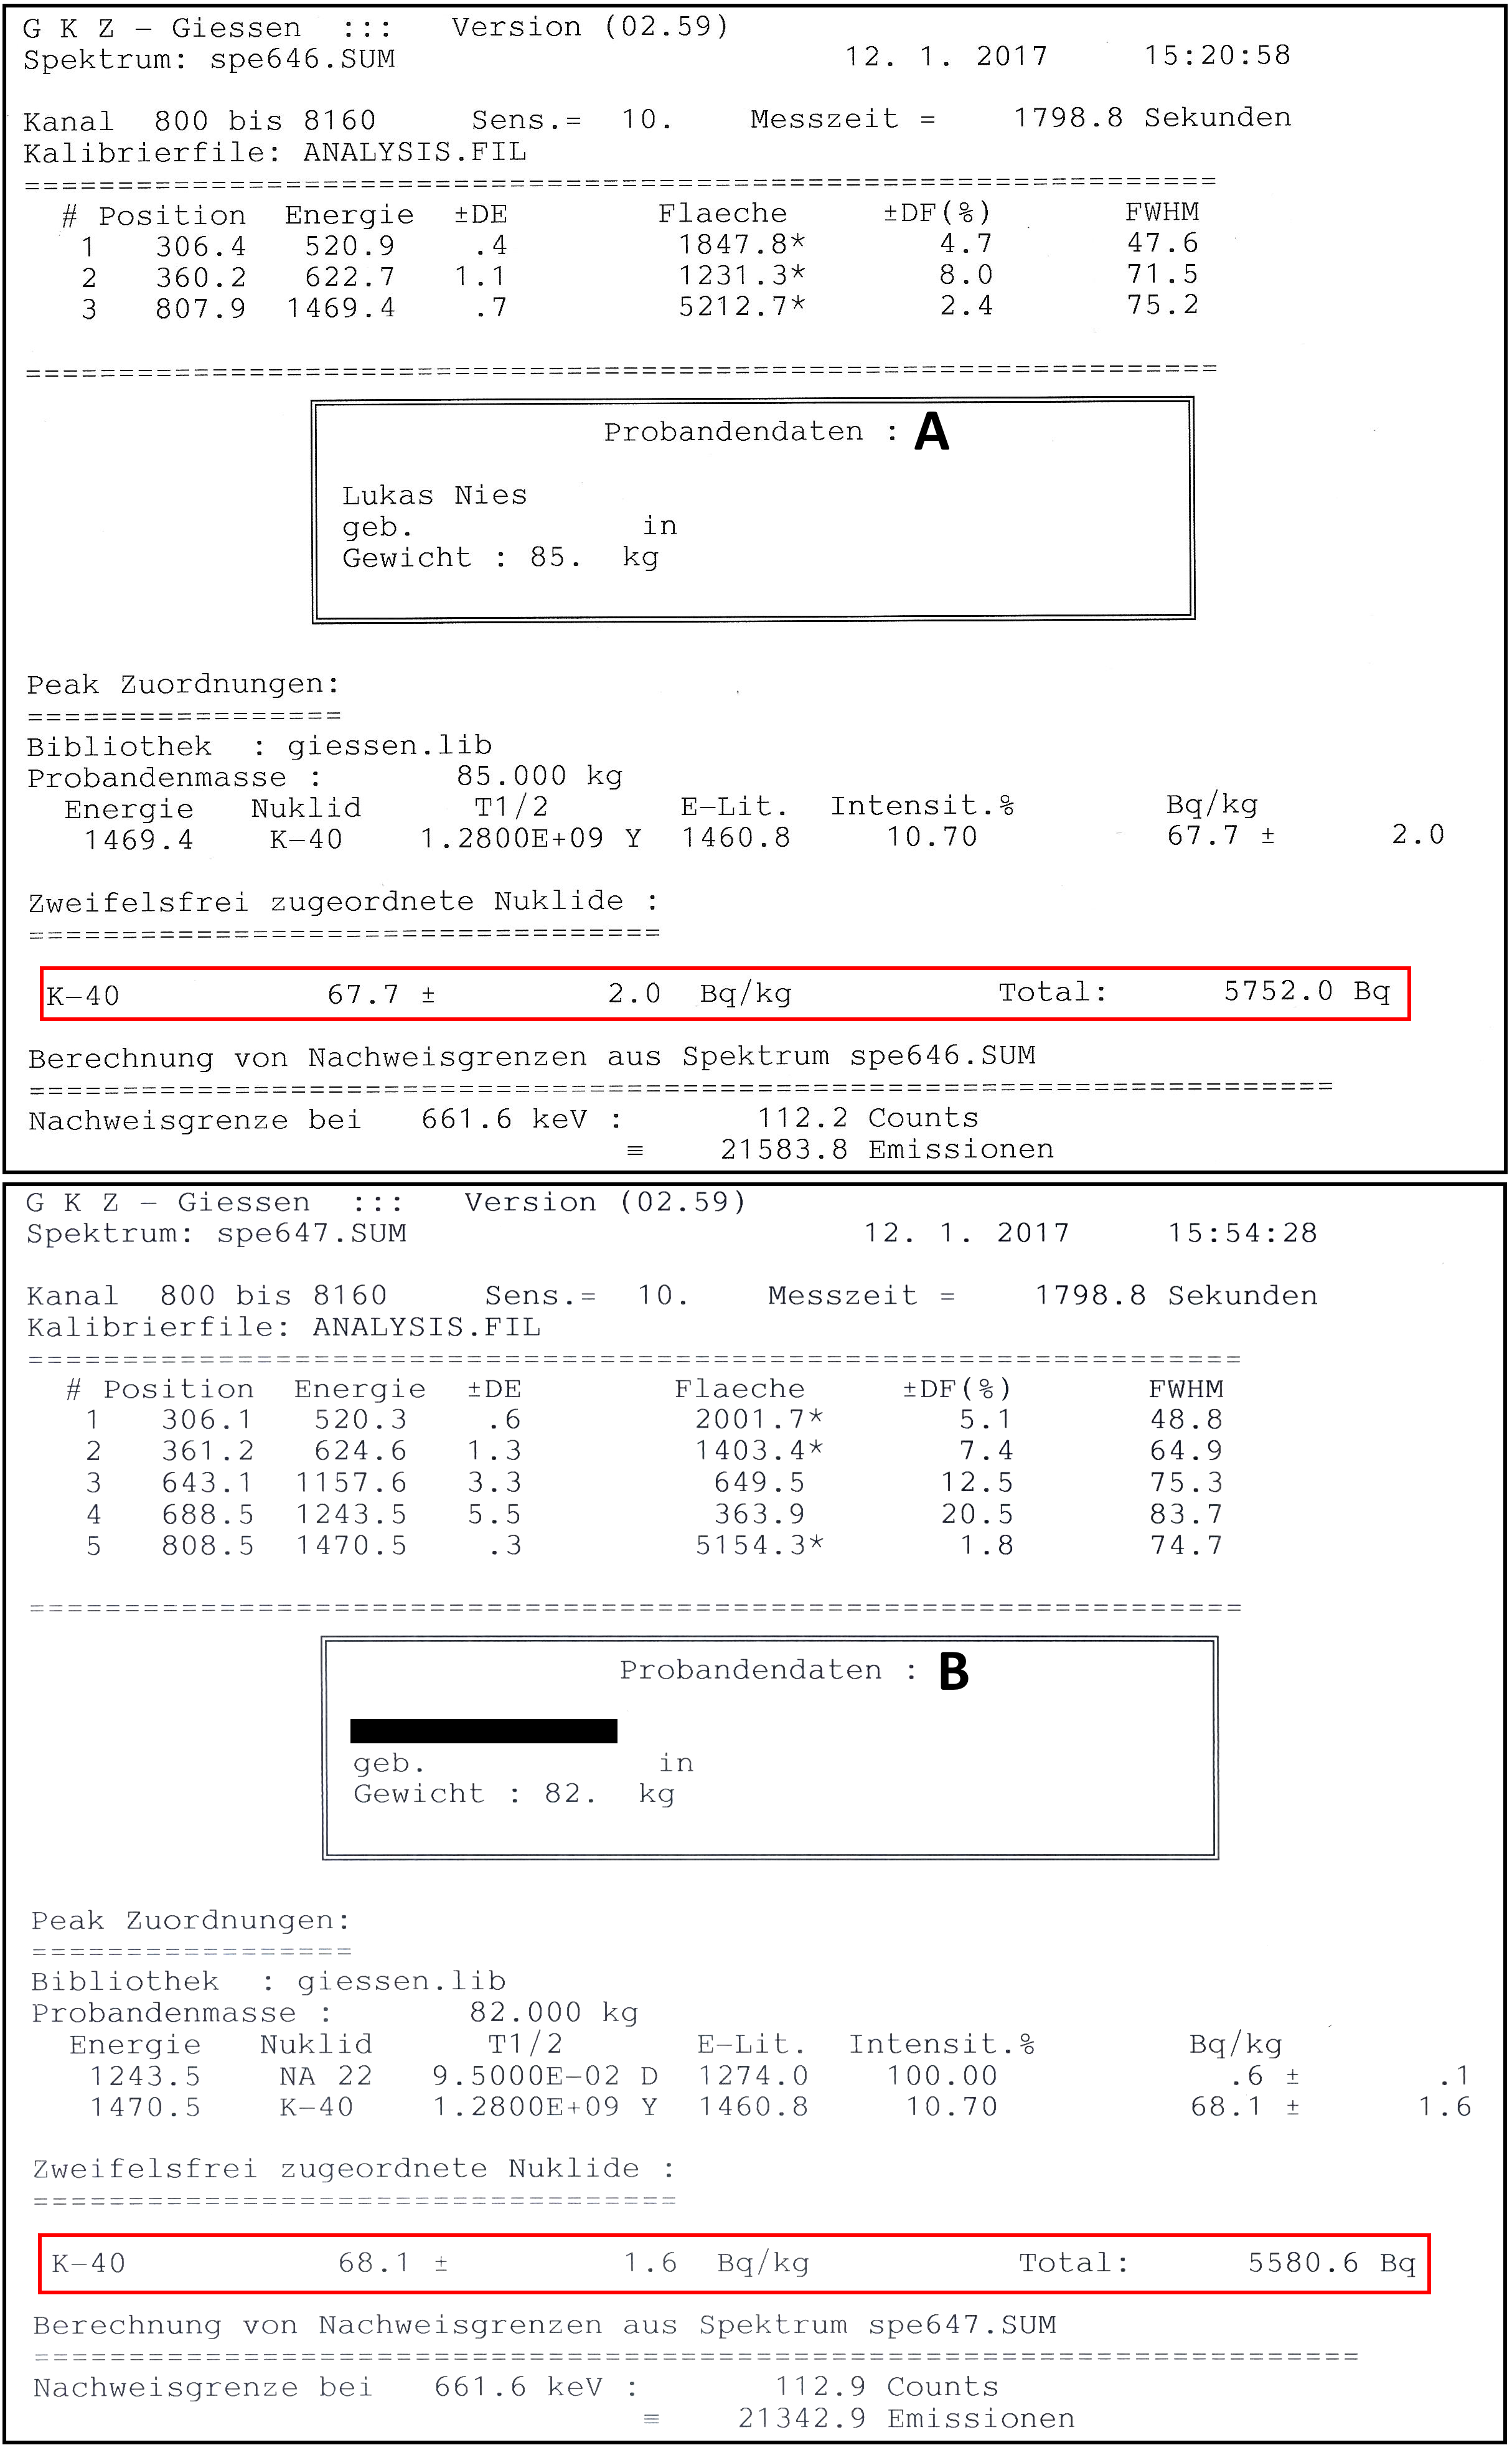
\includegraphics[width=0.85\linewidth]{./20161216/probanden.png}
	\caption[Ganzk"orperz"ahler]{Ergebnisse der Ganzk"orperz"ahlungen beider Probanden.}
	\label{fig:probanden}
\end{figure}

\clearpage

\section{Literatur- und Bildverzeichnis}
\bibliographystyle{plain}
\bibliography{./bib}

\listoffigures

\end{appendices}
















  



\end{document}  